%==============================================================================
% tento soubor pouzijte jako zaklad
% this file should be used as a base for the thesis
% Autoři / Authors: 2008 Michal Bidlo, 2018 Jaroslav Dytrych
% Kontakt pro dotazy a připomínky: dytrych@fit.vutbr.cz
% Contact for questions and comments: dytrych@fit.vutbr.cz
%==============================================================================
% kodovani: UTF-8 (zmena prikazem iconv, recode nebo cstocs)
% encoding: UTF-8 (you can change it by command iconv, recode or cstocs)
%------------------------------------------------------------------------------
% zpracování / processing: make, make pdf, make clean
%==============================================================================
% Soubory, které je nutné upravit: / Files which have to be edited:
%   xhanak33_water_level_monitoring-20-literatura-bibliography.bib - literatura / bibliography
%   xhanak33_water_level_monitoring-01-kapitoly-chapters.tex - obsah práce / the thesis content
%   xhanak33_water_level_monitoring-30-prilohy-appendices.tex - přílohy / appendices
%==============================================================================
%\documentclass[]{fitthesis} % bez zadání - pro začátek práce, aby nebyl problém s překladem
%\documentclass[english]{fitthesis} % without assignment - for the work start to avoid compilation problem
%\documentclass[zadani]{fitthesis} % odevzdani do wisu a/nebo tisk s barevnými odkazy - odkazy jsou barevné
%\documentclass[english,zadani]{fitthesis} % for submission to the IS FIT and/or print with color links - links are color
%\documentclass[zadani,print]{fitthesis} % pro černobílý tisk - odkazy jsou černé
%\documentclass[english,zadani,print]{fitthesis} % for the black and white print - links are black
\documentclass[zadani,cprint]{fitthesis} % pro barevný tisk - odkazy jsou černé, znak VUT barevný
%\documentclass[english,zadani,cprint]{fitthesis} % for the print - links are black, logo is color
% * Je-li práce psaná v anglickém jazyce, je zapotřebí u třídy použít 
%   parametr english následovně:
%   If thesis is written in english, it is necessary to use 
%   parameter english as follows:
%      \documentclass[english]{fitthesis}
% * Je-li práce psaná ve slovenském jazyce, je zapotřebí u třídy použít 
%   parametr slovak následovně:
%   If the work is written in the Slovak language, it is necessary 
%   to use parameter slovak as follows:
%      \documentclass[slovak]{fitthesis}
% * Je-li práce psaná v anglickém jazyce se slovenským abstraktem apod., 
%   je zapotřebí u třídy použít parametry english a enslovak následovně:
%   If the work is written in English with the Slovak abstract, etc., 
%   it is necessary to use parameters english and enslovak as follows:
%      \documentclass[english,enslovak]{fitthesis}

% Základní balíčky jsou dole v souboru šablony fitthesis.cls
% Basic packages are at the bottom of template file fitthesis.cls
% zde můžeme vložit vlastní balíčky / you can place own packages here

% Kompilace po částech (rychlejší, ale v náhledu nemusí být vše aktuální)
% Compilation piecewise (faster, but not all parts in preview will be up-to-date)
% \usepackage{subfiles}

% Nastavení cesty k obrázkům
% Setting of a path to the pictures
%\graphicspath{{obrazky-figures/}{./obrazky-figures/}}
%\graphicspath{{obrazky-figures/}{../obrazky-figures/}}

%---rm---------------
\renewcommand{\rmdefault}{lmr}%zavede Latin Modern Roman jako rm / set Latin Modern Roman as rm
%---sf---------------
\renewcommand{\sfdefault}{qhv}%zavede TeX Gyre Heros jako sf
%---tt------------
\renewcommand{\ttdefault}{lmtt}% zavede Latin Modern tt jako tt

% vypne funkci šablony, která automaticky nahrazuje uvozovky,
% aby nebyly prováděny nevhodné náhrady v popisech API apod.
% disables function of the template which replaces quotation marks
% to avoid unnecessary replacements in the API descriptions etc.
\csdoublequotesoff

% =======================================================================
% balíček "hyperref" vytváří klikací odkazy v pdf, pokud tedy použijeme pdflatex
% problém je, že balíček hyperref musí být uveden jako poslední, takže nemůže
% být v šabloně
% "hyperref" package create clickable links in pdf if you are using pdflatex.
% Problem is that this package have to be introduced as the last one so it 
% can not be placed in the template file.
\ifWis
\ifx\pdfoutput\undefined % nejedeme pod pdflatexem / we are not using pdflatex
\else
  \usepackage{color}
  \usepackage[unicode,colorlinks,hyperindex,plainpages=false,pdftex]{hyperref}
  \definecolor{hrcolor-ref}{RGB}{223,52,30}
  \definecolor{hrcolor-cite}{HTML}{2F8F00}
  \definecolor{hrcolor-urls}{HTML}{092EAB}
  \hypersetup{
	linkcolor=hrcolor-ref,
	citecolor=hrcolor-cite,
	filecolor=magenta,
	urlcolor=hrcolor-urls
  }
  \def\pdfBorderAttrs{/Border [0 0 0] }  % bez okrajů kolem odkazů / without margins around links
  \pdfcompresslevel=9
\fi
\else % pro tisk budou odkazy, na které se dá klikat, černé / for the print clickable links will be black
\ifx\pdfoutput\undefined % nejedeme pod pdflatexem / we are not using pdflatex
\else
  \usepackage{color}
  \usepackage[unicode,colorlinks,hyperindex,plainpages=false,pdftex,urlcolor=black,linkcolor=black,citecolor=black]{hyperref}
  \definecolor{links}{rgb}{0,0,0}
  \definecolor{anchors}{rgb}{0,0,0}
  \def\AnchorColor{anchors}
  \def\LinkColor{links}
  \def\pdfBorderAttrs{/Border [0 0 0] } % bez okrajů kolem odkazů / without margins around links
  \pdfcompresslevel=9
\fi
\fi
% Řešení problému, kdy klikací odkazy na obrázky vedou za obrázek
% This solves the problems with links which leads after the picture
\usepackage[all]{hypcap}

% Informace o práci/projektu / Information about the thesis
%---------------------------------------------------------------------------
\projectinfo{
  %Prace / Thesis
  project={BP},            %typ práce BP/SP/DP/DT/DR  / thesis type (SP = term project)
  year={2019},             % rok odevzdání / year of submission
  date=\today,             % datum odevzdání / submission date
  %Nazev prace / thesis title
  title.cs={Vestavěný systém pro monitorování výšky vodní hladiny},  % název práce v češtině či slovenštině (dle zadání) / thesis title in czech language (according to assignment)
  title.en={Embedded System for Water Level Monitoring}, % název práce v angličtině / thesis title in english
  %title.length={14.5cm}, % nastavení délky bloku s titulkem pro úpravu zalomení řádku (lze definovat zde nebo níže) / setting the length of a block with a thesis title for adjusting a line break (can be defined here or below)
  %Autor / Author
  author.name={Jiří},   % jméno autora / author name
  author.surname={Hanák},   % příjmení autora / author surname 
  %author.title.p={Bc.}, % titul před jménem (nepovinné) / title before the name (optional)
  %author.title.a={Ph.D.}, % titul za jménem (nepovinné) / title after the name (optional)
  %Ustav / Department
  department={UPSY}, % doplňte příslušnou zkratku dle ústavu na zadání: UPSY/UIFS/UITS/UPGM / fill in appropriate abbreviation of the department according to assignment: UPSY/UIFS/UITS/UPGM
  % Školitel / supervisor
  supervisor.name={Václav},   % jméno školitele / supervisor name 
  supervisor.surname={Šimek},   % příjmení školitele / supervisor surname
  supervisor.title.p={Ing.},   %titul před jménem (nepovinné) / title before the name (optional)
  %supervisor.title.a={Ph.D.},    %titul za jménem (nepovinné) / title after the name (optional)
  % Klíčová slova / keywords
  keywords.cs={Vestavěný systém, měření vzdálenosti, STM32, návrh DPS, nádrž, voda, ESP8266, ČSN EN 60 529, HAL}, % klíčová slova v českém či slovenském jazyce / keywords in czech or slovak language
  keywords.en={Embedded system, distance measuring, STM32, PCB design, tank, water, ESP8266, ČSN EN 60 529, HAL}, % klíčová slova v anglickém jazyce / keywords in english
  %keywords.en={Here, individual keywords separated by commas will be written in English.},
  % Abstrakt / Abstract
  abstract.cs={Tato práce se zabývá návrhem a realizací vestavěného systému pro monitorování výšky vodní hladiny. Účelem systému je řízení napouštění nádrže na základě výšky vodní hladiny. V první řadě je věnována pozornost přehledu stávajících měřicích technik a výběru vhodných měřicích prvků pro daný scénář. Vestavěný systém staví na bezkontaktních snímačích TFmini a JSN-SR04T-2.0. Řízení systému obstarává mikrokontrolér řady STM32F0 od firmy STMicroelectronics programovaný v jazyce C s využitím abstraktní vrstvy HAL. Naměřené výsledky jsou odesílány přes Wi-Fi SoC ESP8266EX na demonstrační server v jazyce Python.}, % abstrakt v českém či slovenském jazyce / abstract in czech or slovak language
  abstract.en={This work is dealing with the design and implementation of an embedded water level monitoring system. The purpose of the system is to control the filling of a tank based on the water level. First of all, the attention is given to the survey of existing measurement techniques and selection of the appropriate sensing elements for a given scenario. In fact, the embedded system is using TFmini and JSN-SR04T-2.0 contactless sensors. The system is controlled by STM32F0 microcontroller from STMicroelectronics programmed in C using HAL abstraction layer. The measured results are sent via Wi-Fi SoC ESP8266EX to the Python server that is used for processing and demonstratiton purposes.}, % abstrakt v anglickém jazyce / abstract in english
  %abstract.en={An abstract of the work in English will be written in this paragraph.},
  % Prohlášení (u anglicky psané práce anglicky, u slovensky psané práce slovensky) / Declaration (for thesis in english should be in english)
  declaration={Prohlašuji, že jsem tuto bakalářskou práci vypracoval samostatně pod vedením pana Ing.~Václava Šimka
Uvedl jsem všechny literární prameny a publikace, ze kterých jsem čerpal.},
  %declaration={I declare that I have prepared this Bachelor´s/Master´s/dissertation thesis independently, under the supervision of ...
% ... provided me with further information.
% I listed all of the literary sources and publications that I have used.},
  % Poděkování (nepovinné, nejlépe v jazyce práce) / Acknowledgement (optional, ideally in the language of the thesis)
  %acknowledgment={\todo{V této sekci je možno uvést poděkování vedoucímu práce a těm, kteří poskytli odbornou pomoc (externí zadavatel, konzultant, apod.).}},
  %acknowledgment={Here it is possible to express thanks to the supervisor and to the people which provided professional help
%(external submitter, consultant, etc.).},
  % Rozšířený abstrakt (cca 3 normostrany) - lze definovat zde nebo níže / Extended abstract (approximately 3 standard pages) - can be defined here or below
  %extendedabstract={Do tohoto odstavce bude zapsán rozšířený výtah (abstrakt) práce v českém (slovenském) jazyce.},
  %faculty={FIT}, % FIT/FEKT/FSI/FA/FCH/FP/FAST/FAVU/USI/DEF
  faculty.cs={Fakulta informačních technologií}, % Fakulta v češtině - pro využití této položky výše zvolte fakultu DEF / Faculty in Czech - for use of this entry select DEF above
  faculty.en={Faculty of Information Technology}, % Fakulta v angličtině - pro využití této položky výše zvolte fakultu DEF / Faculty in English - for use of this entry select DEF above
  department.cs={Ústav počítačových systémů}, % Ústav v češtině - pro využití této položky výše zvolte ústav DEF nebo jej zakomentujte / Department in Czech - for use of this entry select DEF above or comment it out
  department.en={Department of Computer Systems} % Ústav v angličtině - pro využití této položky výše zvolte ústav DEF nebo jej zakomentujte / Department in English - for use of this entry select DEF above or comment it out
}

% Rozšířený abstrakt (cca 3 normostrany) - lze definovat zde nebo výše / Extended abstract (approximately 3 standard pages) - can be defined here or above
%\extendedabstract{Do tohoto odstavce bude zapsán výtah (abstrakt) práce v českém (slovenském) jazyce.}

% nastavení délky bloku s titulkem pro úpravu zalomení řádku - lze definovat zde nebo výše / setting the length of a block with a thesis title for adjusting a line break - can be defined here or above
%\titlelength{14.5cm}


% řeší první/poslední řádek odstavce na předchozí/následující stránce
% solves first/last row of the paragraph on the previous/next page
\clubpenalty=10000
\widowpenalty=10000

% checklist
\newlist{checklist}{itemize}{1}
\setlist[checklist]{label=$\square$}

\setlength{\parskip}{0pt}

% begin vlastni upravy
\usepackage{amsmath}
\usepackage{siunitx}
\usepackage{array}
\usepackage{lscape}
\usepackage{xfrac}
\usepackage{float}

\sisetup{detect-all}
\makeatletter
\providecommand\add@text{}
\newcommand\tagaddtext[1]{%
  \gdef\add@text{$#1$\gdef\add@text{}}}% 
\renewcommand\tagform@[1]{%
  \maketag@@@{\llap{\add@text\quad}(\ignorespaces#1\unskip\@@italiccorr)}%
}
\makeatother

% nastaveni tabulek
\setlength{\tabcolsep}{10pt}
% \renewcommand{\arraystretch}{1.5}
\usepackage{booktabs}
\renewcommand{\arraystretch}{1.3}
\newcommand{\ra}[1]{\renewcommand{\arraystretch}{#1}}

\newcommand{\unit}[1]{\ensuremath{\, \mathrm{#1}}}
\usepackage{multirow}
\usepackage{multicol}
% end vlastni upravy

\newcommand{\io}[1]{\textit{#1}}
\newcommand{\conn}[2]{\texttt{#1#2}}
\newcommand{\company}[1]{{#1}}
\newcommand{\ip}[1]{\texttt{#1}}
\newcommand{\sw}[1]{\texttt{#1}}
\newcommand{\norm}[1]{\texttt{#1}}
\newcommand{\block}[1]{\textit{#1}}
\newcommand{\cmd}[1]{\textcolor{blue}{\texttt{#1}}}

\begin{document}
  % Vysazeni titulnich stran / Typesetting of the title pages
  % ----------------------------------------------
  \maketitle
  % Obsah
  % ----------------------------------------------
  {\hypersetup{hidelinks}\tableofcontents}
  
  % Seznam obrazku a tabulek (pokud prace obsahuje velke mnozstvi obrazku, tak se to hodi)
  % List of figures and list of tables (if the thesis contains a lot of pictures, it is good)
  \ifczech
    \renewcommand\listfigurename{Seznam obrázků}
  \fi
  \ifslovak
    \renewcommand\listfigurename{Zoznam obrázkov}
  \fi
  % \listoffigures
  
  \ifczech
    \renewcommand\listtablename{Seznam tabulek}
  \fi
  \ifslovak
    \renewcommand\listtablename{Zoznam tabuliek}
  \fi
  % \listoftables 

  \ifODSAZ
    \setlength{\parskip}{0.5\bigskipamount}
  \else
    \setlength{\parskip}{0pt}
  \fi

  % vynechani stranky v oboustrannem rezimu
  % Skip the page in the two-sided mode
  \iftwoside
    \cleardoublepage
  \fi

  % Text prace / Thesis text
  % ----------------------------------------------
  \chapter{Úvod}

    % využití, Proč je třeba měřit. Co vše se dá ovládat, co vše se dá dat získat, vyvodit.
    Pokračující období sucha v~roce 2019 vede zahrádkáře k~budování nádrží na dešťovou vodu či studny pro přístup k~vodě podzemní. Pro pečlivé hospodaření s~životodárnou tekutinou je žádoucí mít neustálý přehled o~jejích zásobách. Ke zmíněnému účelu je v~této práci navržen vestavěný systém pro monitorování výšky vodní hladiny, který na základě její úrovně může řídit čerpání nebo odčerpávání vody.

    % metody měření
    Práce uvádí do problematiky měření vzdálenosti mezi dvěma objekty v~rozsahu několika metrů oproti referenčnímu bodu. Jsou zmíněny rovněž metody, které nesouvisí přímo s~měřením vzdálenosti mezi dvěma body, avšak lze s~jejich pomocí měřit výšku vodní hladiny.

    % návrh systému
    Vestavěný systém je rozdělen na dvě části - řídicí a podpůrnou, kde první zmíněná část je řízena mikroprocesorem \io{STM32F030CCT6} od firmy \company{STMicroelectronics}, jenž zajišťuje měření výšky vodní hladiny pomocí optického snímače vzdálenosti \io{TFmini}, ultrazvukového snímače vzdálenosti \io{JSN-SR04T-2.0}, teplotního snímače \io{MCP9808} pro korekci naměřených hodnot ultrazvukovým snímačem a čidly limitního stavu hladiny \io{KSL-35-PP}. Podpůrná část obstarává napájení celého systému a zajišťuje spojení s~vnějším světem pomocí Wi-Fi. Obsahuje rovněž tzv. solid state relé, pomocí kterého je řízeno spínání přívodu jednofázového čerpadla. Celý systém je navržen pro stupeň krytí \ip{IP67} dle normy \norm{ČSN EN 60 529}, čehož je docíleno umístěním jednotlivých komponent do instalačních krabic vyhovujících požadovanému stupni krytí a využitím tzv. vývodek pro vyvedení kabelů ze zmíněných krabic.

    % implementace
    Obslužný firmware systému je implementován v~jazyce C s~využitím knihovny HAL (\textit{Hardware Abstract Layer}) vyvíjenou firmou \company{STMicroelectronic}. Systém je řízený dle konfigurace, která mimo jiné definuje připojení k~síti Wi-Fi, adresy serveru, kam jsou hodnoty naměřené snímači odesílány, a limitní úrovně vodní hladiny. 

    % testování
    V~rámci práce byl vestavěný systém spolu se snímači testován na odběr proudu v~klidovém a aktivním režimu. Bylo provedeno testovací měření jednotlivých snímačů pro ověření jejich přesnosti pro účely vestavěného systému. V~rámci testování požadovaného stupně krytí \ip{IP67} byl dle požadavků normy \norm{ČSN EN 60 592} vestavěný systém ponořen do vody do hloubky jednoho metru na dobu třiceti minut.

\chapter{Metody měření výšky vodní hladiny}

    Měření vzdálenosti je z~pohledu automatizace velice důležitý aspekt. V~dnešní době můžeme systémy měřící vzdálenost nalézt v~mnoha oblastech: v~autonomním autě pro udržování bezpečných rozestupů mezi vozidly, ve výrobních linkách, kdy se pomocí výšky určuje množství konkrétního média v~nádobě, v~letadlech pro určování výšky a v~mnoha dalších. Každá aplikace má své specifické požadavky na měřicí systém, ať z~pohledu maximální měřené vzdálenosti, přesnosti, nebo schopnosti měřit v~náročných podmínkách, jako jsou extrémní teploty, tlak či agresivní médium.
    V~dnešní době se díky pokročilým senzorům naskýtá mnoho možností, jak měřit vzdálenost mezi dvěma objekty. V~obecné rovině lze existující principy rozdělit do tří základních skupin:
    
    \begin{itemize}
        \item \bf Mechanické \rm -- založeno na principu pohybu částí měřicího systému. V zásadě se jedná o~specifické metody pro měření výšky kapalin.
        \item \bf Fyzikální \rm -- kdy princip spočívá v~měření konkrétní fyzikální veličiny. Zvláštní kategorií založenou na fyzikálních veličinách je kategorie \bf bezkontaktní\rm.  
        \item \bf Bezkontaktní \rm -- většina bezkontaktních metod měří dobu odezvy na vyslaný signál, ať akustický, optický, či rádiový.
    \end{itemize}

    Část zde popsaných metod není univerzální, neboť reflektují specifické fyzikální a chemické vlastnosti vody. Jelikož je cílem prostřednictvím vestavěného systému monitorovat výšku vodní hladiny a na jejím základě řídit přečerpávání vody do nádrže, jsou zde uvedeny pouze vybrané relevantní metody, kdy je možné hodnoty měřených veličin reprezentovat na elektrické či obvodové úrovni takovým způsobem, aby je bylo možné v~rámci vestavěného systému dále zpracovat.

    \section{Metody založené na fyzikálních veličinách}
        Metody popsané v~této kapitole se opírají především o~fyzikální veličiny a zákony, a chemické vlastnosti vody. Lze předpovědět, že tyto metody jsou závislé na teplotě vody, neboť s~teplotou se mění její hustota, jež je znázorněna na grafu~\ref{img:density}, dále na atmosférickém tlaku a na obsahu nečistot. Poněvadž obsah nečistot není předem známý, jelikož je proměnlivý dle prostředí, je nutné u~těchto metod počítat s~určitým zkreslením výsledků měření.

        \begin{figure*}[h]
            \centering
            \includegraphics[width=\linewidth]{obrazky-figures/water_density.pdf}
            \caption{Závislost hustoty vody na teplotě pro tzv. Standard Mean Ocean Water~\cite{tables}.}
            \label{img:density}
        \end{figure*}

        \subsubsection{Měření hydrostatického tlaku}
            \label{sec:hydro}
            Díky zemské gravitaci se ve vodním sloupci s~jeho narůstající hloubkou přímou úměrou zvyšuje hydrostatický tlak, ze kterého lze dle vzorce~\ref{eq:hydro} vypočítat jeho výšku. Pro měření výšky vodního sloupce v~plném rozsahu kapacity nádrže je nutné hydrostatický tlak měřit u~dna nádrže, neboť umístění senzoru slouží jako referenční bod měření.

            \begin{samepage}
                \begin{gather}
                    \label{eq:hydro}
                    h = \dfrac{p}{\rho\cdot g}
                    \intertext{kde}
                    \begin{tabular}{>{$}r<{$}@{\qquad}p{12cm}}
                        p & je měřený hydrostatický tlak kapaliny\\
                        \rho & představuje hustotu kapaliny\\
                        g & je tíhové zrychlení ($g=9,81\unit{m\cdot s^{-2}}$)\\
                    \end{tabular}\nonumber
                \end{gather}
            \end{samepage}
            
            Měření tlaku je ve své podstatě velice jednoduché, neboť je dnes již velký výběr tlakoměrů. Většina tlakoměrů se řadí k~diferenciálním, jež snímají tlak vzduchu nad hladinou a tlak vody v~místě, kde je senzor umístěn. Existují však i tlakoměry absolutní, které měří tlak vody oproti nulovému tlaku (vakuu). Tlak je možno měřit přímo, kdy je senzor ponořen do nádrže, nebo je zabudovaný do jeho stěny. Při nepřímém způsobu měření se pak uplatní membrána, která chrání samotný senzor před korozivními účinky vody. Je možné měřit i pomocí tzv. probublávání, kdy je do potrubí situovaného nad hladinou zakončeného svislou trubicí zespodu otevřenou u~dna nádrže, vháněn vzduch, jehož tlak je předmětem měření. Po vyrovnání tlaku vzduchu v~potrubí a hydrostatického tlaku na jeho konci začne vzduch unikat v~podobě bublinek.
            
            Přesnost zmíněné metody je přímo závislá na použitém senzoru pro snímání tlaku a aktuální hustotě vody~\cite{dado}. Jelikož jsou senzory vyráběné do určitého maximálního tlaku, je třeba při jeho výběru brát na tento fakt zřetel. 

        \subsubsection{Měření konduktivity}
            % https://www.fd.cvut.cz/personal/janes/elektrotechnika1/Prednaskyprezentace/Predn05_Vodivost_PevneL_Kapaliny_Plyny.pdf
            Mezi význačné vlastnosti, kterými voda disponuje, patří její elektrická vodivost, která je závislá na koncentraci elektrolytů. 
            Ačkoli destilovaná voda je téměř nevodivá ($0,5\unit{\mu S\cdot cm^{-1}}$), pitná voda vykazuje více než tisícinásobnou vodivost $0,5$--$1\unit{mS\cdot cm^{-1}}$~\cite{conductivity}. Přehled měrné vodivosti některých druhů vod je uveden v~tabulce~\ref{table:waters}. Uvážíme li, že zbytek nádrže je vyplněn vzduchem, který je za normálních podmínek nevodivý~\cite{gas_conductivity}, lze detekovat, zdali jsou dvě elektrody umístěné do předem určené výšky zatopeny (je vytvořen vodivý spoj) či nikoli. Vodivost pitné vody je způsobena koncentrací iontů rozpuštěných látek~\cite{water_conductivity}, a kvůli tomu by při průchodu stejnosměrného elektrického proudu docházelo k~elektrolýze. Aby k~ní nedocházelo, je třeba snímat sepnutí proudem střídavým. Jelikož voda zapříčiňuje korozi, je třeba vybrat korozivzdorné elektrody.

            \begin{table*}[h]\centering
                \begin{tabular}{@{}rcc@{}}\toprule
                    \textbf{Měrná vodivost}                 && \textbf{Médium}\\
                    \midrule
                    $0,05\unit{\mu S\cdot cm^{-1}}$         && Čistá voda\\
                    $0,5\unit{\mu S\cdot cm^{-1}}$          && Destilovaná voda\\
                    $0,1$--$10\unit{\mu S\cdot cm^{-1}}$    && Deionizovaná voda\\
                    $1$--$80\unit{\mu S\cdot cm^{-1}}$      && Demineralizovaná voda\\
                    $10\unit{\mu S\cdot cm^{-1}}$           && Horská voda\\
                    $0,5$--$1\unit{mS\cdot cm^{-1}}$        && Pitná voda\\
                    $53\unit{mS\cdot cm^{-1}}$              && Mořská voda\\
                    \bottomrule
                \end{tabular}
                \caption{Závislost měrné vodivosti na měřeném médiu~\cite{conductivity}.}
                \label{table:waters}
            \end{table*}

        \subsubsection{Měření elektrické kapacity}
            \label{sec:capacitance}

            Další možností pro monitorování výšky vodní hladiny je měření elektrické kapacity kondenzátoru. Jelikož je pro měření uvažována studna či nádrž, předpokládá se, že stěny nejsou z~vodivého materiálu.

            Jak již bylo zmíněno v~předešlém odstavci, lze považovat vodu za vodivé médium. Díky tomu můžeme sestrojit kondenzátor, ve kterém bude figurovat voda jako elektroda o~proměnné velikosti, přičemž druhá je tvořena kupříkladu vodivou tyčí obalenou nevodivou vrstvou, která bude sloužit jako dielektrikum~\cite{dado}. 
            Takto sestrojený kondenzátor bude se změnami výšky vodní hladiny měnit svoji kapacitu. Se známou měrnou permitivitou dielektrika lze ze změřené kapacity dle vzorce~\ref{eq:capacitor} vypočítat samotnou výšku vodní hladiny.  
            
            \begin{samepage}
                \begin{gather}
                    \label{eq:capacitor}
                    C=C_0+\dfrac{2\cdot\pi\cdot\varepsilon_0\cdot\varepsilon_r}{\ln\left(\dfrac{D}{d}\right)}\cdot h 
                    \intertext{kde}
                    \begin{tabular}{>{$}r<{$}@{\qquad}p{12cm}}
                        C_0 & je stálá kapacita vedení\\
                        \varepsilon_0 & je permitivita vakua ($\varepsilon_0 = 8,854\,187\,818\cdot10^{-12}\unit{H\cdot m^{-1}}$)\\
                        \varepsilon_r & je měrná permitivita izolace\\
                        d & je průměr samotné elektrody\\
                        D & je průměr elektrody s~izolací\\
                        h & je hloubka ponořené části\\
                    \end{tabular}\nonumber
                \end{gather}
            \end{samepage}

            Předností této metody je především nezávislost na teplotě vody, okolnímu tlaku ani na obsahu nečistot. Avšak kvůli ulpívání vodního kamene a jiných usazenin na měřicí elektrodě se zmenšuje nezávisle na výšce vodní hladiny povrch elektrody (vnějšího pláště).

    \section{Metody založené na pohyblivých částech}
        V~této části jsou popsány metody, které vyžadují specifický pohyb určité části systému pro dosažení měření. Tyto metody jsou kvůli pohyblivým částem z~dlouhodobého hlediska pro přesné měření nevhodné, neboť hrozí jejich přirozené opotřebení a v~důsledku zanedbání údržby i jejich vyřazení z~provozu. Také je potřeba pro dosažení určitého stupně krytí vynaložit větší úsilí při konstrukci vodotěsného spojení pevné části a pohyblivého prvku. Jejich základním kamenem je plovák, který se spolu s~vodní hladinou pohybuje nahoru a dolů. Jejich použití je však vhodné, když teplota měřené kapaliny může nabývat velkého rozsahu, neboť žádná měřicí část není přímo závislá na teplotě, a tudíž přesnost měření je stále konstantní.

        \subsubsection{Měření úhlu ramena s~plovákem vůči stěně nádrže}
            \label{sec:plovak}
            Jednou z~možností využití plováku je jeho umístění na rameno, které je pevně spojeno s~osou snímače náklonu, nejčastěji pomocí otočného potenciometru, kdy pohyb plováku otáčí s~jeho osou a tím nastavuje odpor, nebo pomocí Hallovy sondy\footnote{Senzor pro měření magnetického pole využívající tzv. Hallova jevu.}. Poloha snímače, respektive osy ramena, představuje referenční bod měřicího aparátu. Jak je znázorněno na obrázku~\ref{img:arm}, úhel svírající stěnu nádrže a ramene je přímo závislý na výšce vodní hladiny. Uvážíme-li nejjednodušší příklad, kdy je osa ramene umístěna při stěně nádrže v~úrovni maximální výšky vodní hladiny a jeho délka je větší nebo rovna maximální výšce vodní hladiny $H$, je možné s~využitím sinusové věty z~úhlu vypočítat samotnou výšku vodní hladiny dle vzorce~\ref{eq:arm}.

            \begin{samepage}
                \begin{gather}
                    \label{eq:arm}
                    h = H - l \cdot \sin{(90 - \alpha)}
                    \intertext{kde}
                    \begin{tabular}{>{$}r<{$}@{\qquad}p{12cm}}
                        \alpha & je úhel svírající stěnu nádrže a rameno\\
                        H & je maximální výška vodní hladiny\\
                        l & je délka ramene\\
                    \end{tabular}\nonumber
                \end{gather}
            \end{samepage}

            \begin{figure*}[h]
                \centering
                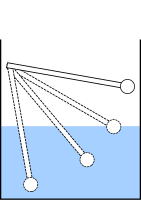
\includegraphics[width=7cm]{obrazky-figures/float.pdf}
                \caption{Princip měření výšky vodní hladiny na základě pohybu plováku připevněného k~rameni.}
                \label{img:arm}
            \end{figure*}

            Tímto postupem dostaneme rozsah měření roven délce ramena za předpokladu, že rameno je kratší, než je maximální výška vodní hladiny. V~opačném případě je rozsah měření roven výšce nádrže, neboť plovák se zastaví o~jeho dno a níže již neklesne.
            Jak vyplývá z~obrázku~\ref{img:arm}, rozsah měřeného úhlu je $90^\circ$, a proto je nezbytné, aby byla nádrž široká minimálně na délku ramene, aby nedocházelo k~jeho zablokování o~protější stěnu nádrže. Při umístění osy ramene do poloviny maximální výšky nádrže se minimální délka ramene zkrátí na polovinu, přičemž rozsah měřeného úhlu již bude $180^\circ$, proto rozsah měření již nyní bude $\pm$ délka ramene. Touto úpravou dosáhneme maximální přesnosti měření, jelikož je v~tomto případě na jednotku změny výšky vodní hladiny způsoben největší pohyb ramene, a tudíž je dosaženo největšího rozdílu úhlu. Docílíme také minimální šířky nádrže z~důvodu zkrácení ramene na minimální mez. 

        \subsubsection{Měření délky měřicího prvku navíjeného pružinou}

            Jedná se o~metodu vycházející z~kombinace principů svinovacího metru, kdy je vzdálenost měřena pomocí značek přesně rozmístěných na měřicím prvku navíjeném pružinou, a detekce pohybu kolečka v~myši, kdy je pohyb přenášen na perforovaný prvek, jenž svými otvory přerušuje proud světelného toku~\cite{mouse}, který je snímán fototranzistorem. Pro určení směru pohybu perforovaného prvku je zařízení vybaveno hned dvěma fototranzistory umístěnými vedle sebe po směru pohybu perforovaného prvku, kdy je směr určen na základě polohy impulzů z~fototranzistorů na časové ose. 
            Měřicí aparatura této metody pro měření výšky vodní hladiny se skládá ze čtyř částí:
            
            \begin{itemize}
                \item \bf Plovák \rm -- dostatečně těžký natolik, aby bez problémů odvíjel měřící pásku z~navíjecího zařízení
                \item \bf Měřicí prvek (páska) \rm -- jež je po předem definované délce pravidelně perforována, může být použit i řetěz
                \item \bf Snímací část \rm -- zdroj světla v~podobě LED\footnote{LED -- Light-Emitting Diode, česky elektroluminiscenční dioda.} a dvojice fototranzistorů, která snímá impulzy
                \item \bf Navíjecí zařízení \rm -- pružina, případně navíjecí buben, jenž udržuje měřící prvek v~napnutém stavu
            \end{itemize}

            Princip metody spočívá v~čítání jednotlivých impulzů z~fototranzistorů. Před uvedením měřicího zařízení do provozu je nutné jej zkalibrovat vůči referenčnímu bodu, který se nachází v~místě snímací části. Kalibrace se provede vynulováním čítače impulzů při minimální nebo maximální výšce vodní hladiny. Způsob kalibrace určuje, zda se měří výška vodní hladiny vůči dnu nádrže nebo od její maximální výšky.

            Nespornou výhodou této metody je, že ji je možné použít pro měření takřka neomezené hloubky. Pro měření ve vyšších hloubkách je ale potřeba také zohlednit váhu měřicí pásky a schopnost navíjecího zařízení ji navinout. Její přesnost závisí na počtu děr v~měřicí pásce na jednotku délky. 

        \subsubsection{Snímání sepnutí jazýčkového kontaktu pomocí magnetu}
            Dvoustavové metody jsou díky své podstatě velice jednoduché a účinné, avšak mají jednu velikou nevýhodu. Tou je jejich indispozice měřit výšku vodní hladiny souvisle. Jejich jediná výstupní informace je, zda vodní sloupec dosáhl předem definované úrovně (pozice, na které je senzor umístěn) či nikoli. Pro přesnější měření výšky vodního sloupce je nezbytné použít více těchto snímačů. V~některých případech, díky absenci řídicí elektroniky, je možné u~těchto snímačů je přímo napojit na spínací prvek, jenž může spínat čerpadlo, nebo jen aktivovat světelnou indikaci signalizující dosažení určité výšky vodního sloupce v~nádrži. 

            Jednou takovou možností je pomocí permanentního magnetu umístěného v~plováku, jenž se pohybuje po svislé vodicí tyči, spínat jazýčkové kontakty. Každý jazýčkový kontakt může mít vyvedeny vlastní vodiče, nebo je možné, pro snížení potřebných kontaktů na řídicí elektronice, mít kontakty zapojené do matice. Ovšem je možné využít i dvouvodičové zapojení mnoha jazýčkových kontaktů v~kombinaci s~rezistory zapojenými do série, kde jednotlivé jazýčkové kontakty spínají jednu elektrodu snímače a konkrétní uzel mezi rezistory, čímž se vytvoří uzavřená smyčka o~určitém odporu.
            Spínací část je možné mít umístěnou uvnitř nádrže, kupříkladu ve vodicí trubce, nebo je možné ji mít upevněnou na vnější stěně (nebrání-li magnetu spínat kontakty). Dle technických možností se magnet pohybuje na krátké ose, řádově centimetry, a spíná jeden kontakt, nebo se může pohybovat v~rámci výšky nádrže a spínat nespočet kontaktů. Výhodou této metody je, že není potřeba řešit korozivzdorné elektrody ani není nutné snímat sepnutí střídavým proudem, aby nedocházelo k~elektrolýze. 

    \section{Metody nevyžadující přímý styk s~kapalinou}
        \label{sec:contactless}
        Velmi pohodlné je monitorování výšky vodní hladiny pomocí bezkontaktních metod, neboť neobsahují žádné mechanické části, které se mohou zadrhnout nebo poškodit, a nejsou přímo vystaveny kontaktu s~vodou. Díky tomu nevyžadují takřka žádnou údržbu a jejich životnost je vysoká. 

        Jejich princip spočívá ve vyslání impulzu, který se od vodní hladiny částečně odrazí a částečně projde do dalšího media, kdy odražený impulz je přijat přijímačem. Vzdálenost vodní hladiny od měřicího zařízení se určí na základě doby mezi vysláním impulzu a jeho následným příjmem podělený dvěma (cesta k~hladině a cesta zpátky) a rychlosti šíření impulzu ve volném prostředí (vzduchu) dle vzorce~\ref{eq:contactless}. Jelikož na jeden vyslaný impuls může dorazit více odražených, přijímač musí být schopen je vyfiltrovat. 

        Bezkontaktní metody, jako jediná kategorie metod snímaní vodní hladiny, vyžadují i minimální hloubku, od které dokáží měřit, neboť pro spolehlivé měření musí mít vysílaný signál určitou dobu trvání, aby byl přijímač schopen jej zachytit. Proto musí být měřená vzdálenost větší než polovina vzdálenosti, kterou stihne urazit impulz od počátku vysílání do skončení vysílání. 

        Při známé vzdálenosti umístění měřicího zařízení od dna, pouhým rozdílem této hodnoty a vypočítané vzdálenosti ze vzorce~\ref{eq:contactless}, dostaneme skutečnou výšku vodní hladiny. Ačkoli tyto metody nezávisí na konkrétních vlastnostech vody (hustota, teplota, vodivost, atd.), přesnost měření je velmi závislá na kompenzaci měřicího zařízení pro konkrétní podmínky, jakými jsou teplota a vlhkost vzduchu, které ovlivňují rychlost šíření vln (podrobněji v~grafech~\ref{img:us_speed} a~\ref{img:light_speed}). Aby se zamezilo absorpci vln ve vodní pěně při napouštění a nechtěných odražených vln od zařízení a potrubí v~nádrži, je vhodné pro měření využít trubici, ve které bude klidná hladina, od které bude docházet ke kolmému odrazu vyslaného impulzu. Dosah této metody závisí na výkonu vysílače a citlivosti přijímače. Z~fyzikálního hlediska dále na absorpci prostředí, odrazivosti překážky a rozptylu vysílaného impulzu. Jejich přesnost měření se pohybuje v~řádech milimetrů.

        \begin{samepage}
            \begin{gather}
                \label{eq:contactless}
                L =\dfrac{c\cdot t}{2}
                \intertext{kde}
                \begin{tabular}{>{$}r<{$}@{\qquad}p{12cm}}
                    c & je rychlost vlnění v~konkrétních podmínkách\\
                    t & je doba mezi odesláním a příjmem impulzu\\
                \end{tabular}\nonumber
            \end{gather}
        \end{samepage}

        \subsubsection{Měření pomocí ultrazvukového vlnění}
            Ultrazvukem je označováno mechanické vlnění nad horní hranicí slyšitelnosti lidského ucha, které je přibližně $20\unit{kHz}$. Maximální měřicí vzdálenost se odvíjí od absorpce zvukové vlny ve vzduchu a odrazivosti překážky. Na základě dat z~tabulky~\ref{table:gas} lze prohlásit, že se zvyšující se frekvencí impulsů a snižující se vlhkostí vzduchu se maximální měřicí vzdálenost zkracuje. Proto je více než vhodné volit pracovní frekvenci co nejnižší. 
            Rychlost mechanického vlnění je především závislá na teplotě, jak dokazuje graf~\ref{img:us_speed}, dále pak na atmosférickém tlaku a vlhkosti, jež ovlivňují rychlost jen částečně. 

            \begin{table*}[h]\centering
                \begin{tabular}{@{}ccccccc@{}}
                    \toprule
                    \multirow{2}{*}{$\varphi\unit{[\%]}$}& \multicolumn{6}{c}{$f\unit{[kHz]}$}\\
                    \cmidrule{2-7}
                        &   1       &   2       &   4       &   6       &   8       &   10      \\
                    \midrule
                    10  &   0,13    &   0,47    &   1,27    &   1,87    &   2,26    &   2,53    \\
                    20  &   0,06    &   0,23    &   0,82    &   1,61    &   2,48    &   3,28    \\
                    40  &   0,03    &   0,10    &   0,38    &   0,84    &   1,45    &   2,20    \\
                    60  &   0,03    &   0,09    &   0,24    &   0,54    &   0,96    &   1,47    \\
                    80  &   0,03    &   0,08    &   0,20    &   0,39    &   0,69    &   1,08    \\

                    \bottomrule
                \end{tabular}
                \caption{Absorpční součinitel $\alpha \cdot 10^2\unit{m^{-1}}$ v~závislosti na relativní vlhkosti vzduchu $\varphi$ a frekvenci mechanického vlnění $f$~\cite{tables}.}
                \label{table:gas}
            \end{table*}

            \begin{figure}[H]
                \centering
                \includegraphics[width=\linewidth]{obrazky-figures/sound_speed.pdf}
                \caption{Rychlost zvuku ve vzduchu v~závislosti na jeho teplotě vypočítána dle vzorce $c = \sqrt{\kappa\cdot R\cdot T}$, kde $\kappa$ je adiabatická konstanta ($\kappa = 1,402$ pro vzduch), $R$ je plynová konstanta ($R=287,05\unit{J\cdot kg^{-1}\cdot K^{-1}}$ pro vzduch), $T$ je termodynamická konstanta ($T= t + 273,15\unit{K}$)~\cite{dado}.}.
                \label{img:us_speed}
            \end{figure}
            %\clearpage

        \subsubsection{Měření pomocí elektromagnetického vlnění}
            \label{sec:el_wave}
            Elektromagnetické vlnění dosahuje, oproti mechanickému, rychlosti světla. Jak je znázorněno na grafu~\ref{img:light_speed}, jeho rychlost není konstantní, neboť se odvíjí od vlnové délky a média, jímž prochází. Rychlost světla se vypočítá dle vzorce~\ref{eq:light_speed}. Pro výpočet indexu lomu pro konkrétní vlnovou délku v~rozsahu $0,2$ -- $2,06\unit{\mu m}$ (viditelné světlo a infračervená oblast) pro suchý vzduch za standardních podmínek ($15^\circ\unit{C}, 101,325\unit{kPa}$ a obsahu $0,03\,\%\,\unit{CO_2}$) platí disperzní vztah~\ref{eq:refractive_index}~\cite{tables}.

            \begin{figure*}[h]
                \centering
                \includegraphics[width=\linewidth]{obrazky-figures/light_speed.pdf}
                \caption{Rychlost elektromagnetického vlnění v~suchém vzduchu v~závislosti na vlnové délce při teplotě $t = 15^\circ \unit{C}$, atmosférickém tlaku $p_0 = 101,325\unit{kPa}$ a obsahu $0,03\,\%\,\unit{CO_2}$.}
                \label{img:light_speed}
            \end{figure*}

            \begin{samepage}
                \begin{gather}
                    \label{eq:light_speed}
                    v~= \dfrac{c}{n}
                    \intertext{kde}
                    \begin{tabular}{>{$}r<{$}@{\qquad}p{12cm}}
                        c & je rychlost světla ve vakuu ($c = 2,997\,924\,580\cdot10^8\unit{m\cdot s}^{-1}$)\\
                        n & je index lomu pro konkrétní médium\\
                    \end{tabular}\nonumber
                \end{gather}
            \end{samepage}

            \begin{samepage}
                \begin{gather}
                    \label{eq:refractive_index}
                    n = 6,4328\cdot 10^{-5} + \dfrac{2,94981\cdot 10^{-2}}{146-\left(\dfrac{1}{\lambda_0}\right)^2} + \dfrac{2,554\cdot 10^{-4}}{41-\left (\dfrac{1}{\lambda_0}\right )^2} + 1
                    \intertext{kde}
                    \begin{tabular}{>{$}r<{$}@{\qquad}p{12cm}}
                        \lambda_0 & je vlnová délka ve vakuu v~$\unit{\mu m}$\\
                    \end{tabular}\nonumber
                \end{gather}
            \end{samepage}

            Teplotní a tlaková korekce se poté dopočítá dle vzorce~\ref{eq:temperature_corr}~\cite{tables}.

            \begin{samepage}
                \begin{gather}
                    \label{eq:temperature_corr}
                    n = (n_{15,\,p_0} - 1)\cdot \dfrac{(1+15\cdot\gamma) \cdot p}{(1 + t \cdot \gamma) \cdot p_0}
                    \intertext{kde}
                    \begin{tabular}{>{$}r<{$}@{\qquad}p{12cm}}
                        n_{15,\,p_0} & index lomu ve vzduchu pro konkrétní vlnovou délku při známé teplotě a tlaku \\
                        \gamma & teplotní součinitel objemové roztažnosti vzduchu $\gamma = 3,670\cdot 10^{-3}\unit{K^{-1}}$\\
                        p_0 & normální atmosférický tlak $p_0 = 101,325\unit{kPa}$\\
                        p & pracovní tlak\\
                        t & pracovní teplota\\
                    \end{tabular}\nonumber
                \end{gather}
            \end{samepage}


            Vyšších frekvencí (řádově GHz) využívá radar\footnote{Radar je anglický akronym pro \it{Radio Detection and Ranging}.}. Na rozdíl od viditelné a infračervené oblasti odrazivost vln závisí na elektrické vodivosti překážky, neboť při dopadu impulzu na vodivou překážku dojde ke zkratu elektrického pole a následnému odrazu. Rychlost šíření vlnění rádiových vln v~konkrétním médiu se stanoví dle vzorce~\ref{eq:light_speed_2}.

            \begin{samepage}
                \begin{gather}
                    \label{eq:light_speed_2}
                    c = \dfrac{c_0}{\sqrt{\mu_r\cdot\varepsilon_r}}
                    \intertext{kde}
                    \begin{tabular}{>{$}r<{$}@{\qquad}p{12cm}}
                    c_0 & je rychlost světla ve vakuu ($c = 2,997\,924\,580\cdot10^8\unit{m\cdot s}^{-1}$)\\
                    \mu_0 & je permeabilita média\\
                    \varepsilon_0 & je permitivita média\\
                    \end{tabular}\nonumber
                \end{gather}
            \end{samepage}

\chapter{Návrh vestavěného systému}
    
    Následující kapitola představuje úvod do problematiky vestavěných systémů a poukazuje na jejich význam v~kontextu dnešního světa. Jsou zde nastíněny nutné předpoklady pro kvalitní řešení hardwarové stránky vestavěného systému pro monitorování výšky vodní hladiny a také jeho návrh jako celku.

    \section{Vestavěný systém}
        %Vestavěný systém je definován dle ESTP (Embedded System Technology Platform) Evropské strategické iniciativy\todo{citace} jako {\it kombinace hardwaru a softwaru, jejímž smyslem je řídit externí proces, zařízení nebo systém.} 
        Vestavěný systém se pro běžné uživatele jeví jako tzv. černá skříňka\footnote{Černá skříňka je kalk z~anglického black box.}, která skrývá svoje vnitřní uspořádání a logiku, avšak navenek vykazuje předem známé chování vůči okolním podmětům. Jejich hlavním účelem je vykonávat určitou svěřenou činnost, nejčastěji bez vnějšího zásahu. V~dnešní době jsou takovéto systémy takřka všudypřítomné, přičemž je možno se s~nimi setkat například v~automatech na kávu, domácích spotřebičích, fotoaparátech, měřicích a komunikačních přístrojích, tiskárnách, výrobních linkách, vesmírných raketách, nebo také v~automobilech. 

        Vesměs vestavěný systém můžeme chápat jako desku plošných spojů (DPS) s~mikrokontrolérem (procesorem) jako řídícím členem a mnoha snímači a prvky pro ovládání nejrůznějších komponent či funkčních bloků, jako jsou spínací relé, elektromotory, reproduktory, či světla. Komunikace s~nimi, na rozdíl od univerzálních počítačů, je zprostředkována především snímači a speciálními komunikačními rozhraními.
    
        Jelikož mají vestavěné systémy předem určenou úlohu, nevzniká potřeba je vybavovat nadbytečně velmi výkonými mikrokontroléry se spoustou periferií, velkou pamětí či celou řadou senzorů. Každá úloha je specifická, a proto je více méně nutné mít pro konkrétní úlohu konkretní vestavěný systém. Může být sestaven z~již dostupných menších systémů (senzory s~komunikačním rozhraním, komunikační moduly, různé adaptéry, atd.), jejichž výhodou je odladěná funkčnost dodávaného systému a díky tomu rychlejší doba návrhu. Na druhou stranu může být realizován jednou či více na míru navrženými a optimalizovanými deskami plošných spojů (rádio, pračka, automobil, dron, atd.), které disponují kompaktními rozměry a v~případě sériové výroby i nižšími náklady na výrobu. Není ovšem nutné se držet jednoho směru, a proto je možné mít vestavěný systém, který kombinuje jejich výhody. Kombinace je vhodná především při realizaci menšího počtu kusů, nebo když dostupné systémy nevyhovují specifickým potřebám.

        Dle grafu~\ref{img:trend_mcu} lze prohlásit, že současný trend přeje vestavěným systémům, kdy počet prodaných mikrokontrolérů meziročně roste v~řádech jednotek procent, částečně i díky rozmachu internetu věcí, kde jeden z~klíčových aspektů technického řešení představují právě vestavěné systémy. Díky stálému poklesu jednotkové ceny mikrokontrolérů jsou tyto systémy čím dál více dostupnější a také rozšířenější.

        \begin{figure*}[h]
            \centering
            \includegraphics[width=\linewidth]{obrazky-figures/mcu_market_history.pdf}
            \caption{Vývoj cen a počet prodaných mikrokontrolérů s~odhadem na další léta (převzato z~\cite{mcu_market_history}).\it\newline
                \newline Millions of Dollars and Units = Miliony dolarů a kusů
                \newline Market = Tržní hodnota
                \newline Units = Počet kusů
                \newline ASP = Průměrná prodejní cena za jeden kus}
            \label{img:trend_mcu}
        \end{figure*}

    \section{Specifikace požadavků na vestavěný systém}
        Monitorování vodní hladiny a přečerpávání vody do zásobní nádrže je ukázková úloha pro vestavěný systém, neboť není vyžadována žádná interakce s~uživatelem a jeho činnost se řídí předem nastavenými pravidly. Dle specifického prostředí a jasně definovaného účelu je nutné u~tohoto vestavěného systému klást důraz především na tyto aspekty:

        \begin{itemize}
            \item \bf Spolehlivost (bezporuchovost) \rm -- očekává se několikaletá životnost, při které by měl systém fungovat celoročně bez výraznějších problémů.
            \item \bf Odolnost vůči vodě \rm -- jelikož se v~tomto případě počítá s~umístěním do blízkosti vodního zdroje, je nutné systém zabezpečit dle normy \norm{ČSN EN 60 529} stupněm krytí \ip{IP67}.
            \item \bf Bezúdržbovost \rm -- od systému je očekáváno autonomní chování, které bude zajišťovat korekci naměřených dat dle aktuálních podmínek (např. atmosferické vlivy) v~místě jeho nasazení. 
            \item \bf Aktuálnost naměřených dat \rm -- systém bude odesílat data v~reálném čase, není od něj vyžadována tvorba statistických ukazatelů z~naměřených údajů.
            \item \bf Rozsah měření výšky vodní hladiny \rm -- stanoven dle prostorových dispozic konkrétní nádrže.
            \item \bf Přesnost měření \rm -- přesnost měření požadovaných údajů musí vyhovovat předem stanoveným požadavkům.
            \item \bf Konektivita \rm -- jelikož se počítá s~využitím serveru, který bude přijímat naměřená data, je třeba zajistit připojení vestavěného systému k~internetové síti. Dále je vhodné mít možnost upravovat konfiguraci použitých snímačů (jejich počet či konkrétní typ) pro měření výšky vodní hladiny.
            \item \bf Jednoduchá instalace \rm -- jelikož není předem známo konkrétní prostřední, je vhodné koncipovat vestavěný systém pro jednoduchou montáž.
            \item \bf Bezpečnost \rm -- systém by měl být odolný proti předvídatelným poruchám (zakrytí výhledu bezkontaktních snímačů, trvale sepnuté/nesepnuté spínače hlídající mezní úrovně hladiny, výpadek elektrického proudu).
            \item \bf Efektivnost \rm -- poněvadž je od systému požadováno nepřetržité monitorovaní, je velmi žádoucí systém navrhnout takovým způsobem, aby byl energeticky nenáročný. 
        \end{itemize}

        Dle výše zmíněných požadavků na vestavěný systém jsem navrhl jeho blokové schéma, jež je uvedeno na obrázku~\ref{img:block_scheme}. Systém je rozdělen na dvě hlavní části - \texttt{řídicí} a \texttt{podpůrnou}, kde jsou jednotlivé aspekty pro funkčnost systému striktně rozděleny.

        \begin{figure*}[h]
            \centering
            \includegraphics[width=\linewidth]{obrazky-figures/scheme.pdf}
            \caption{Blokové schéma vestavěného systému.}
            \label{img:block_scheme}
        \end{figure*}

    \section{Řídicí část vestavěného systému}
        Řídicí část obsahuje jádro systému - desku osazenou mikrokontrolérem a konektory pro připojení různých snímačů, a dále samotné snímače. Schéma zapojení této desky je uvedeno v~příloze~\ref{sec:main_board_scheme}, podklad pro výrobu desky plošného spoje je pak možno nalézt v~příloze~\ref{sec:main_board_pcb}. 

        Styl návrhu desek plošných spojů byl uzpůsoben technice smíšené montáže pouze z~jedné strany, kdy jsou klasické i SMD (\textit{Surface Mount Device}) součástky osazeny pouze z~jedné strany na dvouvrstvý (vícevrstvý) plošný spoj~\cite{book:dps}, a možnosti ručního osazení.

        Návrh plošného spoje probíhal v~otevřeném multiplatformním softwaru KiCad\footnote{\url{www.kicad-pcb.org}}, jenž proces návrhu rozděluje na tvorbu schématu zapojení, přiřazení pouzder použitým součástkám a nákresu DPS. Náhled s~ukázkou vizualizace podoby výsledného návrhu desek plošných spojů lze zobrazit pomocí 3D prohlížeče.

        \subsubsection{Řízení systému - mikrokontrolér}
            Při návrhu plošného spoje je nutné v~prvních chvílích vybrat vhodný mikrokontrolér. Vzhledem k~použitému účelu, není třeba nutně zvolit model s~velkým výkonem a pamětí. Naproti tomu je však žádoucí, aby disponoval dostatečným počtem vhodných komunikačních rozhraní pro připojení snímačů. Kvůli nepřetržitému běhu je příhodné, aby nevykazoval velkou spotřebu elektrické energie. Na základě těchto kritérií jsem zvolil mikrokontrolér \io{STM32F030CCT6} od firmy STMicroelectronics architektury ARM s~32 bitovým jádrem rodiny Cortex-M0. Dle značení STM lze vyčíst, že se jedná o~rodinu \texttt{F0}, jež disponuje menším výkonem a je určena pro nízko nákladové aplikace~\cite{stm:f0}. Nabízí $32\unit{kB}$ paměti SRAM, $256\unit{kB}$ flash paměti, 37 vstupně-výstupních pinů, 6 rozhraní UART, 2 rozhraní pro I$^2$C, 2 pro SPI. Jeho pracovní frekvence je $f_t=48\unit{MHz}$~\cite{stm:datasheet}.

        \subsubsection{Konektivita vestavěného systému}
            Plošný spoj řídicí části disponuje pro připojení snímačů 4 porty komunikačního rozhraní UART, které jsou na desce plošného spoje dostupné prostřednictvím konektorů označených symboly \conn{J}{1}, \conn{J}{2}, \conn{J}{4} a \conn{J}{5}. S~výjimkou konektoru \conn{J}{1} lze u~nich zvolit pro reprezentaci logických úrovní napětí mezi $5\unit{V}$ a $3,3\unit{V}$, k~čemuž slouží zkratové propojky situované nalevo od jednotlivých konektorů. Při návrhu byl brán ohled na tolerované úrovně napětí na pinech mikrokontroléru. V~případě potřeby je možné dané konektory nakonfigurovat jako dva vstupně/výstupní piny s~vlastním napájením a zemí. Dále je k~dispozici konektor \conn{J}{3} sběrnice I$^2$C s~pracovním napětím $3,3\unit{V}$. Pomocí pasivní redukce se dvěma pull-up rezistory a vhodné konfigurace mikrokontroléru je možné získat další rozhraní I$^2$C na konektoru \conn{J}{4}. Deska je také osazena dvěma konektory \conn{J}{6} a \conn{J}{7} pro připojení ponorných kontaktů na sledování mezních stavů vodní hladiny. Dle nastavení firmwaru je možné do každého z~těchto dvou konektorů připojit po jednom ponorném kontaktu, nebo lze využít zapojení do tzv. matice, jak je znázorněno na obrázku~\ref{img:matrix}, kdy je možno sledovat sepnutí až 4 ponorných kontaktů. Rozmístění všech konektorů je možno pozorovat na snímku 3D modelu řídicí desky~\ref{img:main_board_3D}. Z~důvodu snahy o~co nejkompaktnější rozměry desky a ne příliš velkého výběru snímačů vhodných pro monitorování výšky vodní hladiny vybavených rozhraním SPI, nebylo rozhraní SPI bráno v~potaz při návrhu plošného spoje, byť jím je použitý mikrokontrolér vybaven.

            \begin{figure}[h]
                \centering
                
\includegraphics[width=0.6\linewidth]{obrazky-figures/matrix.pdf}
                \caption{Schéma zapojení ponorných kontaktů pro sledování až 4 mezních stavů vodní hladiny.}
                \label{img:matrix}
            \end{figure}

            Pro programování a ladění je deska vybavena konektorem \conn{J}{8}. K~indikaci klíčových událostí a stavů je deska plošného spoje vybavena 2 LED \conn{D}{1} a \conn{D}{2}. Propojení s~podpůrnou částí je řešeno prostřednictvím konektoru \conn{J}{9}, přičemž komunikace je zprvu zprostředkována rozhraním UART. Jelikož vedení může být ovlivněno nepříznivými vlivy, je komunikace následně převedena na RS-485, čehož je docíleno pomocí diferenciálního sběrnicového přijímače-vysílače \io{SN75176A}. Díky tomuto převodu je možné z~hlediska komunikace umístit hlavní části systému až do vzdálenosti $1\,200\unit{m}$~\cite{book:embedded_1}. 

            \begin{figure*}[h]
                \centering
                \includegraphics[width=0.8\linewidth]{obrazky-figures/main_board_3D.pdf}
                \caption{3D model řídicí desky (pro lepší čitelnost značení nejsou v~modelu zahrnuty THT součástky).}
                \label{img:main_board_3D}
            \end{figure*}

            \subsubsection{Komunikační rozhraní UART}
                Univerzální asynchronní vysílač-přijímač (anglicky \textit{Universal Asynchronous Receiver and Transimitter}, zkráceně UART) je hardwarové zařízení, jež zprostředkovává asynchronní sériovou komunikaci s~volitelnou přenosovou rychlostí, tzv. baud rate. Pro plnou obousměrnou komunikaci využívá binární signál na dvou sériových linkách označovaných Tx pro vysílání a Rx pro příjem. Ve chvíli, kdy není přenášena žádná zpráva, nabývá signál logické \cmd{1}, jakožto klidového stavu. V~opačném případě je přenášen datový rámec, znázorněný na obrázku~\ref{img:uart}, který sestává ze start bitu, 7--8 datových, volitelně jednoho paritního a jednoho až dvou stop bitů.~\cite{book:embedded_1}

                \begin{itemize}
                    \item \bf Start bit \rm -- označuje začátek přenosu datového rámce změnou z~klidové úrovně na logickou \cmd{0}, využívá se k~synchronizaci hodin přijímače s~hodinami vysílače.
                    \item \bf Datové bity \rm -- bity přenášené zprávy.
                    \item \bf Paritní bit \rm -- většinou volitelné zabezpečení korektnosti datového rámce schopné detekovat jednu chybu. Dle konfigurace je možné nastavit lichou nebo sudou paritu.
                    \item \bf Stop bit \rm -- ukončuje datový rámec změnou do klidové úrovně, z~níž může začít další komunikace
                \end{itemize}

                \begin{figure*}[h]
                    \centering
                    
\includegraphics[width=0.8\linewidth]{obrazky-figures/uart.pdf}
                    \caption{Ukázka asynchronního sériového datového rámce UART~\cite{book:embedded_2}.}
                    \label{img:uart}
                \end{figure*}

            \subsubsection{Komunikační rozhraní I$^2$C}
                Komunikační rozhraní I$^2$C (\textit{Inter-Intergrated Communication}) je synchronní sériové poloduplexní sběrnicové rozhraní, jež ke komunikaci využívá dvě obousměrné linky, a to SDA (\textit{Serial Data}) pro přenos dat a SCL (\textit{Serial Clock}) pro přenos hodinového signálu. Jelikož se při komunikaci počítá s~otevřeným kolektorem a klidovým stavem v~logické \cmd{1}, musí být obě linky připojeny k~externím pull-up rezistorům, typicky s~napětím $3,3\unit{V}$ až $5\unit{V}$~\cite{book:elec}.
                
                U~I$^2$C není žádný centrální prvek, který by řídil komunikaci, všechna připojená zařízení ke sběrnici jsou si rovna. Proto je nutné pro komunikaci využívat adresování. 

                Komunikace je tvořena rámci o~velikosti 8 bitů a potvrzením ze strany přijímače. Zahajuje ji dočasný tzv. master generováním tzv. startovací podmínky, tj. vytvoření sestupné hrany na SDA ve chvíli, kdy je SCL v~úrovni H. Poté přenáší 7 adresových bitů zařízení, se kterým chce komunikovat a bit značící, zda chce z~něj číst nebo do něj zapisovat, přes SDA, přičemž jejich vzorkování ze strany ostatních zařízení připojených ke sběrnici probíhá výhradně při náběžné hraně SCL. Po odeslání těchto bitů čeká na potvrzení ze strany přijímače o~shodě adres. V~závislosti na požadovaném směru toku dat master vysílá datové rámce, nebo je přijímá. Po dokončení přenosu dat master generuje tzv. ukončovací podmínku náběžné hrany na SDA při SCL v~úrovni H.~\cite{book:embedded_1}

                I$^2$C umožňuje adresovat adresou o~velikosti 7 nebo 10 bitů. Pro 7bitovou adresu platí postup výše, pro 10bitovou jsou posílány 2 adresové rámce, přičemž první má prefix \cmd{11110} následovanými 2 nejvíce významnými bity adresy a bitem pro indikaci čtení-zápisu. Druhý adresový rámec poté obsahuje 8 nejméně významných bitů adresy. Oba uvedené způsoby adresování jsou uvedeny na obrázku~\ref{img:iic}.

                \begin{figure*}[h]
                    \centering
                    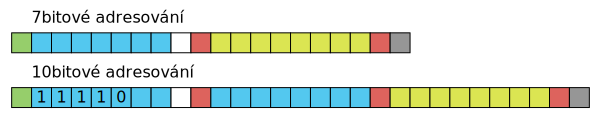
\includegraphics[width=\linewidth]{obrazky-figures/i2c.pdf}
                    \caption{Ukázka 7bitového a 10bitového adresování komunikačního rozhraní I$^2$C~\cite{book:embedded_2}. Startovací podmínka je zvýrazněna zeleně, adresové bity modře, bit určující čtení/zápis bíle, potvrzující bit červeně, datové bity žlutě a ukončující podmínka šedě.}
                    \label{img:iic}
                \end{figure*}

            \subsubsection{Komunikační rozhraní RS-485}
                Pro spolehlivou komunikaci na delší vzdálenost je nutné použít jiné komunikační rozhraní oproti již dříve zmíněným, jelikož by mohlo docházet ke ztrátě kvality signálu, zvláště při vyšších přenosových rychlostech.

                RS-485 je diferenciální rozhraní schopné komunikovat na vzdálenost až $1\,200\unit{m}$, přičemž maximální počet přijímacích zařízení je omezen na 32. Je možné jej implementovat jako poloduplexní dvouvodičové vedení, nebo plně duplexní čtyřvodičové vedeni.
                Maximální přenosová rychlost na vzdálenost $12\unit{m}$ je $35\unit{Mbit \cdot sec^{-1}}$, avšak při vzdálenosti $1\,200\unit{m}$ činí maximální přenosová rychlost pouze $100\unit{kb\cdot s^{-1}}$. Pro zamezení odrazů signálu je třeba, aby oba konce vedení byly ukončeny tzv. terminátory.~\cite{book:elec} 

            \subsubsection{Zatížitelnost řídicí části}
                Z~podpůrné do řídicí částí je přivedeno napětí $5,5\unit{V}$, které je pro napájení mikrokontroléru a připojených snímačů převedeno pomocí měniče \io{MCP1826S-5002E/DB} na $5\unit{V}$ a \io{MCP1826S-3302E/DB} na $3,3\unit{V}$. Oba zmíněné měniče jsou dimenzovány na výstupní proud $1\,000\unit{mA}$~\cite{io:mcp}. Vzhledem k~maximálnímu odběru mikrokontroléru, který je $120\unit{mA}$~\cite{stm:datasheet}, odběru posuvníku logické úrovně \io{SN74LV1T34} $7\unit{mA}$~\cite{io:sn74}, který převádí logickou úroveň přijatých dat z~podpůrné části na $3,3\unit{V}$, a dalších částí systému, je možné připojit snímače pracující s~$3,3\unit{V}$ v~hraničním případě až do odběru $850\unit{mA}$. Maximální proudové omezení snímačů pracujících s~napětím $5\unit{V}$, které je sníženo o~odběr diferenciálních sběrnicových vysílačů-přijímačů \io{SN75176A} a jejich ukončovací rezistory, jež odpovídá $50\unit{mA}$~\cite{io:sn75}, činí $900\unit{mA}$. 

        \subsubsection{Výběr senzorů}
            \label{sec:sensors}

            Smyslem prováděných měření není ani tak zjišťování výšky vodní hladiny samotné, jako spíše objemu vody ve studni či nádrži. Je zvykem, že studny mají tvar postaveného válce, a proto není problém z~výšky dopočítat objem vody dle vzorce $V = \pi \cdot r^2 \cdot v$. Avšak u~nádrží může vzniknout problém, neboť kromě již zmíněného postaveného válce může mít tvar kvádru či válce ležatého, případně s~vypouklým dnem. Pomineme-li tvar kvádru, jehož závislost objemu na výšce je lineární funkce, bylo by pro monitorování objemu nutné data z~dálkových snímačů převádět dle převodní tabulky nebo pomocí funkce. Stejná situace nastane, pokud ve studni (nádrži) budou znatelnější překážky, jako je potrubí nebo jakákoliv konstrukce.

            Bezkontaktní snímače je nutné vybrat s~ochranou \ip{IP67}, nebo je vhodně umístit do takového prostředí, v~němž je tato ochrana zajištěna, aniž by byla narušena jejich schopnost spolehlivě měřit. Dálkové snímače, jež nejsou určeny pro průmyslové použití, neobsahuje zabudovaný teploměr pro korekci naměřených dat. Je na zváženou, zda pro dosažení co nejvyšší přesnosti měření vestavěný systém teplotním snímačem vybavit. Jak znázorňuje tabulka~\ref{table:compare}, při použití ultrazvukového snímače bez teplotní korekce může být rozdíl v~naměřené vzdálenost při teplotách $T_0=0^\circ\unit{C}$, $T_2=25^\circ\unit{C}$ a doby letu signálu $t=15\unit{ms}$ až $14,1\unit{cm}$. Při využití elektromagnetického vlnění s~vlnovou délkou $\lambda=850\unit{nm}$ při stejném rozdílu teplot a při době letu signálu $t=20\unit{ns}$, kdy pro teplotu $T_0=5^\circ\unit{C}$ odpovídá vzdálenost $2,997\unit{m}$, je rozdíl v~naměřené vzdálenosti jen $\Delta_L = 72,4\unit{\mu m}$.

            Na základě těchto údajů lze prohlásit, že pro měření využívající elektromagnetické vlnění není potřeba brát v potaz teplotní korekci. U~snímačů využívající ultrazvukové vlnění to již nelze říci.

            \begin{table*}[h]\centering
                \begin{tabular}{@{}ccccccc@{}}
                    \toprule
                    \multirow{2}{*}{\phantom{a}T$\unit{[^\circ C]}$\phantom{a}}& \multicolumn{6}{c}{Doba letu signálu$\unit{[ms]}$}\\
                    \cmidrule{2-7}
                        &   2       &   5       &   10      &   15      &   20      & 25\\
                    \midrule
                    0   &   0,331   &   0,829   &   1,658   &   2,487   &   3,316   & 4,144\\
                    5   &   0,335   &   0,836   &   1,673   &   2,510   &   3,346   & 4,182\\
                    10  &   0,338   &   0,844   &   1,688   &   2,532   &   3,376   & 4,220\\
                    15  &   0,341   &   0,852   &   1,703   &   2,554   &   3,405   & 4,257\\
                    20  &   0,343   &   0,859   &   1,717   &   2,576   &   3,435   & 4,293\\
                    25  &   0,347   &   0,866   &   1,732   &   2,598   &   3,464   & 4,330\\
                    \bottomrule
                \end{tabular}
                \caption{Závislost stanovené vzdálenosti překážky v~metrech při využití vzorce~\ref{eq:contactless} na konkrétní teplotě a doby letu ultrazvukového signálu.}
                \label{table:compare}
            \end{table*}

            Za účelem dosažení co největší spolehlivosti se nabízí osadit systém několika snímači různého druhu. Na základě této myšlenky a již zmíněných okolností jsem pro vestavěný systém vybral následující snímače: 
            \begin{itemize}
                \item TFmini
                \item JSN-SR04T-2.0
                \item MCP9808 
                \item KSL-35-PP
            \end{itemize}

            \subsubsection{Optický snímač vzdálenosti TFmini}

                K~bezkontaktnímu měření vzdálenosti pomocí metody měření letu světelného paprsku popsaného v~sekci~\ref{sec:el_wave} je možné použít \io{TFmini}, který se vyznačuje nízkou cenou, malou velikostí a vysokým výkonem. Díky jeho schopnosti měřit vzdálenost v~rozsahu 0,3--$12\unit{m}$, dostatečně pokrývá aplikaci vestavěného systému, přičemž maximální absolutní chyba měření do $6\unit{m}$ odpovídá $\pm 6\unit{cm}$, v~rozsahu 6--$12\unit{m}$ je již relativní chyba $\pm 1\unit{\%}$. Vyzařovací úhel činí $3^\circ$, přičemž je schopen detekovat odražené paprsky až do úhlu $1,15^\circ$ vůči ose detekční čočky.~\cite{sensor:lidar}

                Komunikační rozhraní je tvořeno UART, přes který lze \io{TFmini} dle požadavků nakonfigurovat. Ve výchozím nastavení posílá s~frekvencí $f = 100\unit{Hz}$ rámce o~velikosti 9 bytů, kde první 2 byty označují začátek rámce hodnotou \cmd{0x59}, následuje dvojce naměřenou vzdáleností, dále dvojice, jež určuje kvalitu odraženého signálu, byte určující v~jakém rozsahu bylo měření provedeno, rezervní byte a nakonec byte s~kontrolním součtem.

                Mezi konfigurovatelné položky patří výstupní formát dat, frekvence měření, jednotka měření (milimetr nebo centimetr), měřicí mód, prahové hodnoty měření, spoušť měření a baud rate.

                \begin{figure*}[h]
                    \centering
                    \includegraphics[width=0.4\linewidth]{obrazky-figures/lidar.pdf}
                    \caption{LiDAR (\textit{Light Detection And Ranging}) modul pro měření vzdálenosti (převzato z~\cite{shop:lidar}).}
                    \label{img:lidar}
                \end{figure*}

                Jelikož \io{TFmini} není chráněn dostatečným stupněm krytí a pro správnou funkci vyžaduje přímý výhled na vodní hladinu, je nezbytné jej umístit do krabice chráněné krytím \ip{IP67} s~průhledným otvorem.
                
            \subsubsection{Ultrazvukový snímač vzdálenosti JSN-SR04T-2.0}

                Zástupce standardních ultrazvukových modulů pro měření vzdálenosti, avšak vodotěsný, je \io{JSN-SR04T-2.0} s~rozsahem měření 0,2--$6\unit{m}$ a pracovní frekvencí $f_W = 40\unit{kHz}$. Maximální absolutní chyba měření při rozlišení na milimetr činí $\pm 1\unit{cm}$.~\cite{sensor:jsn}

                \begin{figure*}[h]
                    \centering
                    \includegraphics[width=0.6\linewidth]{obrazky-figures/jsn.pdf}
                    \caption{Ultrazvukový vodotěsný modul pro měření vzdálenosti (převzato z~\cite{shop:jsn}).}
                    \label{img:jsn}
                \end{figure*}

                Disponuje třemi pracovními režimy, které se nastaví hodnotou rezistoru \conn{R}{27} na DPS.
                \begin{itemize}
                    \item \bf Analogový režim \rm -- $R_{27}$ není zapojen, měření započne nastavením pinu \texttt{Trig/Tx} minimálně na dobu $10\unit{\mu S}$. Poté proběhne 8 měření, na jejichž základě je na pinu \texttt{Echo/Rx} vygenerován pulz odpovídající měřené vzdálenosti. Pro vyčíslení vzdálenosti je nutné šířku impulzu vynásobit rychlostí zvuku pro dané médium a podělit dvěma.
                    \item \bf Cyklický sériový režim \rm -- $R_{27} = 120\unit{k\Omega}$, měření probíhá automaticky s~frekvencí $f=10\unit{Hz}$. Naměřené hodnoty se posílají v~rámcích o~4 bytech přes komunikační rozhraní UART při baud rate 9600. Rámec začíná bytem \cmd{0xFF}, následuje byte horních 8 bitů naměřené hodnoty, poté byte dolních bitů a nakonec byte s~kontrolním součtem.
                    \item \bf Sériový režim \rm -- $R_{27} = 47\unit{k\Omega}$, měření probíhá obdobně jako u~cyklického sériového režimu, avšak s~rozdílem, že měření je spouštěno vysláním bytu o~hodnotě \cmd{0x55}.
                \end{itemize}                

            \subsubsection{Teplotní snímač MCP9808}
                Teplotní snímač \io{MCP9808} od firmy \company{Microchip Technology Inc.} je zástupce digitálních teploměrů v~podobě integrovaného obvodu. Jeho rozsah měření činí $-40^\circ\unit{C}$ až $+125^\circ\unit{C}$, přičemž na rozsahu $-20^\circ\unit{C}$ až $100^\circ\unit{C}$ je absolutní odchylka měření $\Delta_M=\pm0,5^\circ\unit{C}$. Snímač komunikuje přes I$^2$C rozhraní s~volitelnou 7 bitovou adresou v~rozsahu \cmd{0x18} až \cmd{0x1F} přivedením na příslušné piny zvolené logické úrovně. Mezi základní konfiguraci patří volitelné rozlišení mezi $0,5^\circ\unit{C}$, $0,25^\circ\unit{C}$, $0,125^\circ\unit{C}$ a $0,0625^\circ\unit{C}$. Dále také limit teplotního okna a limit kritické teploty, jejichž překročení je signalizováno patřičnými bity v~teplotním registru a v~případě překročení limitu kritické teploty je také nastaven pin \texttt{Alert} do úrovně \cmd{H}. Maximální odběr snímače činí $400\unit{\mu A}$.~\cite{sensor:mcp}

                Snímač je k~systému připojen formou modulu \io{ADAFRUIT 1782}, jenž je znázorněn na obrázku~\ref{img:mcp}.
                \begin{figure*}[h]
                    \centering
                    \includegraphics[width=0.3\linewidth]{obrazky-figures/mcp.pdf}
                    \caption{Modul \io{ADAFRUIT 1782} osazený teplotním snímačem \io{MCP9808} (převzato z~\cite{shop:mcp}).}
                    \label{img:mcp}
                \end{figure*}

            \subsubsection{Snímač limitního stavu hladiny KSL-35-PP}
                \io{KSL-35-PP} je čidlo pro snímání mezní výšky hladiny kapaliny schopné dle prodejní specifikace spínat výkon $10\unit{W}$ při maximálním proudu $I_{max}=500\unit{mA}$~\cite{shop:ksl}.
                \begin{figure*}[h]
                    \centering
                    \includegraphics[width=0.35\linewidth]{obrazky-figures/pk.pdf}
                    \caption{Čidlo: hladiny kapalin KSL-35-PP (převzato z~\cite{shop:ksl}).}
                    \label{img:pk}
                \end{figure*}

    \section{Podpůrná část vestavěného systému}
        Podpůrná část obstarává napájení celého systému a zajišťuje spojení s~vnějším světem pomocí Wi-Fi, a proto je příhodné pro využití plného potenciálu systému ji umístit v~dosahu dostatečně kvalitního signálu. Je vybavena také konektorem pro řízení čerpadla, které bude na základě výšky vodní hladiny spínáno. Schéma zapojení desky plošného spoje obsažené v~podpůrné části je zahrnuto v~příloze~\ref{sec:support_board_scheme}, samotná deska plošného spoje je v~příloze~\ref{sec:support_board_pcb}. Její 3D vizualizace je znázorněna na obrázku~\ref{img:support_board_3D}.

        \begin{figure*}[h]
            \centering
            \includegraphics[width=0.6\linewidth]{obrazky-figures/support_board_3D.pdf}
            \caption{3D model podpůrné desky (pro lepší čitelnost značení nejsou v~modelu zahrnuty THT součástky).}
            \label{img:support_board_3D}
        \end{figure*}

        \subsubsection{Spojení se serverem pomocí Wi-Fi}
            Ke komunikaci s~vnějším světem dle standardů IEEE802.11 b/g/n je deska plošného spoje podpůrné části osazena Wi-Fi modulem \io{ESP-12E} s~platformou \io{ESP8266EX} pracující v~pásmu $2,4\unit{GHz}$~\cite{io:esp8266}, jehož funkcionální blokový diagram je uveden na obrázku~\ref{img:esp8266}. Tento modul je vybaven anténou ve formě cesty na DPS a všemi potřebnými součástmi pro navázání spojení~\cite{io:esp12}. Modul byl vybrán především na základě jeho možnosti přímého osazení na desku plošného spoje. Jeho průměrná spotřeba činí $80\unit{mA}$, avšak při maximálním zatížení může dosahovat až $230\unit{mA}$. Ačkoli disponuje 32 bitovým mikrokontrolérem Tensilica L106, jenž především řídí Wi-Fi komunikaci, není pro potřeby systému více využit. 

            \begin{figure*}[h]
                \centering
                \includegraphics[width=\linewidth]{obrazky-figures/esp8266.pdf}
                \caption{Funkcionální blokový diagram SoC (\textit{System on Chip}) \io{ESP8266EX} (převzato z~\cite{io:esp8266}).}
                \label{img:esp8266}
            \end{figure*}

        \subsubsection{Řízení napouštění nádrže spínáním přívodu čerpadla}
            Při realizaci obvodu pro spínání zátěže, v~našem případě čerpadla, je nutné stanovit jeho maximální výkon, který se většinou pohybuje od $500\unit{W}$ až po $1\,000\unit{W}$, avšak nejsou výjimkou čerpadla i o~výkonu $1\,500\unit{W}$. Proto je patřičné spínací obvod dimenzovat minimálně na tento výkon. Vzhledem k~požadavku na spolehlivost systému jsem při návrhu spínacího obvodu hledal takové řešení, které by neobsahovalo mechanické části, jako jsou relé či stykače. Na základě této úvahy bylo zvoleno tzv. solid state relé (SSR), jež pro spínání využívá polovodičových prvků. Jeho výhody oproti klasickému relé jsou následující~\cite{book:embedded_1}:
            
            \begin{itemize}
                \item delší životnost
                \item větší spolehlivost
                \item rychlejší spínání
                \item lepší mechanická stabilita
                \item odolný vůči vibracím
                \item nedochází k~odrazům jazýčků při sepnutí
                \item menší elektromagnetické rušení
                \item tišší provoz
                \item při spínání nevytváří elektrický oblouk
            \end{itemize}

            Systém je proto vybaven jednofázovým \io{SSR-2528RD3}, které je schopno spínat zátěž až do $25\unit{A}$ při napětí v~rozmezí $24$--$280\unit{V}\ $AC. Je možné jej ovládat signálem o~napětí v~rozsahu $3$--$32\unit{V}\ $DC~\cite{io:ssr}, jenž je vyveden z~DPS prostřednictvím konektoru \conn{J}{3}. 

        \subsubsection{Napájení vestavěného systému}
            Kvůli účelu samotného systému je vyžadováno, aby bylo k~dispozici napětí $230\unit{V}$ střídavých, které bude spínáno jakožto napájení čerpadla. Proto je možné, a také vhodné, využít tento zdroj stálé energie na úkor napájení systému z~baterií pro dlouhodobý a bezúdržbový provoz.
            Napájení je tudíž řešeno pomocí externího zdroje \io{TRACO Power TIW 12-112 }, na jehož vstupu je zmíněných $230\unit{V}$ střídavých a na výstupu $12\unit{V}$ stejnosměrných, které je připojeno pomocí svorkovnice \conn{J}{1} na desku. Kvůli napěťovým měničům \io{MCP1826S-5002E/DB} a \io{MCP1826S-3302E/DB}, jež jsou obsaženy v~obou částech systému pro vytvoření přesných napěťových úrovní, jejichž maximální vstupní napětí je omezeno na $6\unit{V}$~\cite{io:mcp}, a úbytku napětí na vedení mezi částmi systému, jsem zvolil pro rozvod napájení v~systému $5,5\unit{V}$, kterého je dosaženo osazením DPS spínaným zdrojem \io{TPS5420} s~proudovou zatížitelností až 2 ampéry. Díky němu je možno připojit externí zdroj o~výstupním napětí v~rozsahu $10$--$35\unit{V}\ $DC. K~výpočtu poměru hodnot rezistorů \conn{R}{12} a \conn{R}{13}, které určují výstupní napětí spínaného zdroje, slouží vzorec~\ref{eq:source}~\cite{io:tps}. S~využitím odporové řady E24 s~podmínkou $R_{12} \geq 10\unit{k\Omega}$~\cite{io:tps} je tohoto poměru docíleno s~odchylkou $5,5\unit{mV}$ rezistory s~hodnotami $R_{12} = 56\unit{k\Omega}$ a $R_{13} = 16\unit{k\Omega}$.

            \begin{samepage}
                \begin{gather}
                    \label{eq:source}
                    n = \dfrac{U_{out} - U_{ref}}{U_{ref}} = \dfrac{5,5 - 1,221}{1,221} = 3,\overline{504}
                    \intertext{kde}
                    \begin{tabular}{>{$}r<{$}@{\qquad}p{12cm}}
                        U_{out} & je výstupní napětí spínaného zdroje\\
                        U_{ref} & je referenční napětí spínaného zdroje
                    \end{tabular}\nonumber
                \end{gather}
            \end{samepage}

            Uvážíme-li maximální využitelný výkon řídicí části, spotřebu \io{ESP-12E} a \io{SN74LV1T34} pracujících s~napětím $3,3\unit{V}$, dvou \io{SN75176A} a \io{SN74LV1T34} pracujících s~napětím $5\unit{V}$, čtveřici stabilizátorů \io{MCP1826S} a proud potřebný k~řízení SSR, činí celkový výkon systému vyjímaje \io{TPS5420} a externího zdroje dle rovnice~\ref{eq:power_main} $P_{5,5} = 9,8247\unit{W}$. 

            \begin{samepage}
                \begin{gather}
                    \label{eq:power_main}
                    %P = 5 \cdot (1 + 2 \cdot 0.05 + 0.008 + 0.04) + 3.3 \cdot (1 + 0.23 + 0.007) + 4 \cdot 5.5 \cdot 0.00012 = x\unit{W}
                    %ESP 10uA, SN74LV1T34 7mA(8), 
                    P_{5,5} = 3,3 \cdot 1,237 + 5 \cdot 1,148 + 5,5 \cdot 0,00048 = 9,8247\unit{W}
                \end{gather}
            \end{samepage}

            Jak je uvedeno v~rovnici~\ref{eq:power_tsp}, při výstupním napětí $5,5\unit{V}$ je odběr zátěže \io{TPS5420} $I_{TPS5420} = 1,7863\unit{mA}$, jenž s~rezervou se vejde do maximálního odběru $I_{max} = 2\unit{A}$. 

            \begin{samepage}
                \begin{gather}
                    \label{eq:power_tsp}
                    I_{TPS5420} = \dfrac{P}{U} = \dfrac{9,8247}{5,5} = 1,7863\unit{A}
                \end{gather}
            \end{samepage}

            Po připočtení výkonu z~rovnice~\ref{eq:power_main} se ztrátovým výkonem \io{TPS5420} při daném odběru $P_{TPS5420} \approx 0,9718\unit{W}$, je roven maximální souhrnný výkon systému $P_{S} = 10,7964\unit{W}$. Proto je nezbytné vybavit systém externím zdrojem o~výkonu větším, než právě uvedeném. Je nutné zdůraznit, že se jedná o~výkon maximální s~maximální zátěží v~podobě senzorů. Avšak tato situace je krajně nepravděpodobná a reálný výkon systému v~klidovém stavu se senzory uvedenými v~sekci~\ref{sec:sensors} činí $P_{S} = 2,049\unit{W}$.

    \newpage
    \section{Umístění prvků vestavěného systému}
        Pro korektní měření je nutné, aby byla řídicí část umístěna nad horním okrajem nádrže s~přímým výhledem na vodní hladinu. Jak již bylo zmíněno v~kapitole~\ref{sec:contactless}, je vhodné, při použití bezkontaktních snímačů, opatřit systém trubicí situovanou kolmo k~hladině, jež bude spojovat vodní hladinu a snímače, aby se zamezilo tvorbě vodní pěny, která by mohla pohlcovat vyslané ultrazvukové impulzy. Pro zdokonalení odrazu elektromagnetických impulzů je žádoucí, aby na hladině plovala neprůhledná překážka, která může mít podobu polystyrenové koule situované uvnitř již zmíněné trubice.

        Vestavěný systém, již ze své podstaty, se bude nacházet v~blízkosti vodního zdroje, a proto je nutné jeho prvky zabezpečit dle normy \norm{ČSN EN 60 529} stupněm krytí \ip{IP67}, při kterém je zařízení chráněno před nebezpečným dotykem jakoukoliv pomůckou, vniknutí prachu i před následky při ponoření do vody na dobu 30 minut do hloubky $1\unit{m}$. Přehled stupňů krytí proti vniknutí vody a požadavky na jejich dosažení je uveden v~tabulce~\ref{table:ip}.

        \begin{table*}[h]\centering
            \begin{tabular}{@{}cp{4cm}p{8.5cm}@{}}
                \toprule
                Stupeň & Ochrana & Specifikace\\
                \midrule
                X5 & chráněno proti tryskající vodě & voda tryskající z~trysek z~libovolného směru proti krytu nesmí způsobit žádné škodlivé účinky\\
                X6 & chráněno proti intenzivně tryskající vodě & voda intenzivně tryskající z~trysek z~libovolného směru proti krytu nesmí způsobit žádné škodlivé účinky\\
                X7 & chráněno proti účinkům dočasného ponoření do vody & při stanoveném tlaku a čase nezpůsobuje množství vody vniklé do zařízení po dočasném ponoření zařízení škodlivé účinky\\
                X8 & chráněno proti účinkům trvalého ponoření do vody & za podmínek dohodnutých mezi výrobcem a odběratelem, které však musí být přísnější než podmínky stanovené pro charakteristickou číslici 7, nesmí množství vody vniklé do zařízení způsobit při jeho trvalém ponoření škodlivé účinky\\
                \bottomrule
            \end{tabular}
            \caption{Vybrané stupně krytí proti vniknutí vody a požadavky na jejich dosažení dle normy \norm{ČSN EN 60 529}~\cite{esp:at}.}
            \label{table:ip}
        \end{table*}

        Pro dosažení požadovaného stupně krytí \ip{IP67} je řídicí deska spolu s~bezkontaktními snímači vzdálenosti a teplotním snímačem umístěna do plastové krabice \io{TG ABS 1212-6-o} zajišťující daný stupeň krytí~\cite{krabice}, přičemž jsou z~ní vyvedeny vývodky\footnote{\url{www.emas.cz/vyvodky}} se stupněm krytí \ip{IP68} pro vyvedení kabelů k~připojení k~podpůrné části a kontaktním snímačům.

        Stejně jako u~řídicí části, je nutné i u~části podpůrné, aby dosahovala stupně krytí \ip{IP67}, neboť není vyloučeno, že bude umístěna mimo dosah vodního zdroje. Proto je rovněž umístěna do krabice \io{TG ABS 1212-6-o} vyhovující stupněm krytí \ip{IP67}.

        Nákres celého systému, demonstrující rozmístění jednotlivých prvků, je uveden na obrázku~\ref{img:system_scheme}. Výsledná podoba vestavěného systému je uvedena v příloze~\ref{sec:fotky}.

        \begin{figure*}[h]
            \centering
            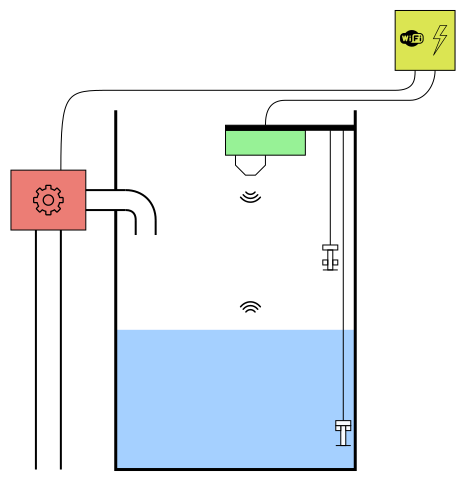
\includegraphics[width=0.8\linewidth]{obrazky-figures/system.pdf}
            \caption{Nákres aplikace vestavěného systému pro monitorování výšky vodní hladiny. Řídicí část, která zodpovídá za naměřené hodnoty, je zvýrazněna zeleně, podpůrná část žlutě a ovládané čerpadlo červeně.}
            \label{img:system_scheme}
        \end{figure*}

\chapter{Implementace firmwaru vestavěného systému}
    Firmware pro řízení mikrokontroléru \io{STM32F030CCT6} je napsán v~jazyce C s~využitím knihovny HAL (\textit{Hardware Abstract Layer}) vyvíjené firmou \company{STMicroelectronic} pro mikrokontroléry rodiny \io{STM32F0}~\cite{stm:hal}, která poskytuje API (\textit{Application programming interface}) pro práci s~mikrokontrolérem a jeho periferiemi, díky které je firmware přenositelný s~obměnou knihoven i na další řady mikrokontrolérů \io{STM32}.
    
    Nejedná se o~jediný přístup k~psaní firmwaru mikrokontrolérů \io{STM32}, neboť je možné jej vyvíjet bez jakékoli abstrakce pouze s~knihovnou CMSIS (\textit{Cortex Microcontroller Software Interface Standard}), kdy je nutná práce přímo s~registry mikrokontroléru. Jedna z~vyšších abstrakcí, avšak dnes již nevyvíjená, využívá knihovny SPL (\textit{Standard Peripheral Library}). Poslední přístup, který konkuruje HAL, je využití knihoven LL (\textit{Low Level}), které zapouzdřují práci s~registry, ale nikoliv s~takovou mírou abstrakce, jako knihovna HAL~\cite{root}.

    Mikrokontrolér lze připojit k~počítači pomocí ST-LINK od firmy \company{STMicroelectronic}, nebo jiných programátorů od různých firem. ST-LINK slouží nejen jako programátor, ale také jako ladicí nástroj a nyní je již dostupný ve třetí vývojové verzi\footnote{\url{www.st.com/en/development-tools/hardware-development-tools-for-stm32.html\#products}}.

    \section{Inicializace firmwaru pomocí nástroje CubeMX}
        CubeMX na základě uživatelské konfigurace mikrokontroléru a požadovaného přístupu generuje inicializační kód korespondující se zvolenou konfigurací~\cite{stm:cubemx}.
        Při vývoji firmwaru pouze s~knihovnou CMSIS, postrádá využití CubeMX smysl, avšak při práci s~HAL či LL usnadní práci. CubeMX\footnote{\url{www.st.com/en/development-tools/stm32cubemx.html}} je multiplatformní okenní nástroj vyvíjený firmou \company{STMicroelectronic}. Zpřístupňuje databázi prodávaných mikrokontrolérů \io{STM32} a vývojových desek nimi osazených, ve které si lze dle požadavků na jádro, vývojovou řadu, pouzdro, cenu, velikost pamětí a periferii vybrat konkrétní mikrokontrolér. Ke každému mikrokontroléru a vývojovému kitu zobrazuje jeho popis, blokový diagram, odkazy na technické dokumentace a všechny potřebné dokumenty pro vývoj. Nechybí ani odkaz na přímý nákup od výrobce.

        Jak je znázorněno na obrázku~\ref{img:cubemx}, umožňuje interaktivní nastavení požadovaných funkcí na příslušné piny mikrokontroléru. V~další fázi je umožněno použitým komunikačním rozhraním nastavit parametry, jako je baud rate, povolení přerušení, přímý přístup do paměti, či pull-up/pull-down rezistory. Nechybí nastavení časovačů ani vnitřních hodin.

        \begin{figure*}[h]
            \centering
            \includegraphics[width=0.8\linewidth]{obrazky-figures/cubemx.pdf}
            \caption{Interaktivní konfigurace pinů v~prostředí CubeMX.}
            \label{img:cubemx}
        \end{figure*}

        S~jeho využitím byly inicializovány vnitřní hodiny na $f_{clock}=8\unit{MHz}$, časovač \conn{TIM}{6}, rozhraní I$^2$C a UART, a GPIO piny.

        \subsubsection{Programování mikrokontroléru}
            Pro komunikaci s~mikrokontrolérem je vhodný nástroj \sw{STM32CubeProgrammer}\footnote{\url{www.st.com/en/development-tools/stm32cubeprog.html}} od firmy \company{STMicroelectronic}. Nástroj je dostupný jak s~grafickým uživatelským rozhraním, tak i s~rozhraním pro práci v~příkazové řádce, díky čemuž je možné zautomatizovat práci s~mikrokontrolérem na základě příkazů v~programu \texttt{Make} spolu s~překladem kódu. 
            
            \sw{STM32CubeProgrammer} umožňuje čtení, zápis, mazání a verifikaci paměti mikrokontroléru i externích pamětí přes rozhraní \texttt{JTAG} a \texttt{SWD}, poskytuje rozhraní pro zavaděč přes UART, USB DFU, I$^2$C, SPI a CAN~\cite{stm:cubeprog}. 

    \section{Obsluha komunikačních rozhraní}
        Pro správnou funkci systému je nutné zajistit spolehlivou komunikaci, aby nebyl ztracen ani jeden byte informace. Z~tohoto důvodu je veškerá komunikace přes UART řízena na základě přerušení přijatého/odeslaného znaku. Všechna rozhraní UART jsou vybavena pro příjem příchozích zpráv a rovněž i pro odchozí komunikaci strukturou \cmd{Vector\_t}, která zajišťuje dynamicky prostor potřebný pro jejich uchování do doby, než budou zpracovány. 

        Struktura \cmd{Vector\_t} vychází z~datové struktury \texttt{fronta}, kdy tok dat je řízen principem \uv{První dovnitř, první ven}. Je tvořena potřebným množstvím struktur \cmd{Vector\_unit\_t}, z~nichž každá má prostor pro 128 znaků zprávy. Pro případ, že by byla přijata zpráva, která by si vyžádala větší paměťový prostor, něž jaký je pro korektní chod systému únosný, je nastaven limit zprávy na 2048 znaků. Další přijaté znaky jsou zahazovány.

    \section{Implementace obsluhy senzorů}
        I~když je systém vybaven bezkontaktními senzory schopnými měřit s~rozlišením v~řádech milimetrů, samotné měření z~podstaty věci nemůže poskytnout tak přesné výsledky, neboť napouštění nádrže, její vypouštění, či jiné příčiny zvlnění vodní hladiny mohou zkreslovat její výšku. Jedním měřením by mohlo být změřeno chvilkové maximum nebo minimum. Kvůli tomuto jevu je vhodné provést více měření s~drobným časovým rozestupem, na jejichž základě se určí výsledná výška vodní hladiny. Počet měření v~jednom cyklu je možné nastavit položkou \cmd{AVERAGE\_COUNT} v~konfiguraci systému (podrobněji v~sekci~\ref{sec:cfg}).

        Nelze zaručit, že všechny použité senzory budou spolehlivě měřit několik let bez údržby. Může se zanést sklo před \io{TFmini}, nebo usazeniny ve vodě mohou zamezit pohybu kroužku na \io{KSL-35-PP}. I~kvůli těmto jevům je systém vybaven hned třemi různými snímači výšky vodní hladiny, i když je schopen pracovat pouze s~jedním z~nich. Je žádoucí, nastane-li problém s~některým ze snímačů, aby mohly být jeho výsledky vyřazeny z~měření, a nemohl tak svou poruchou vyřadit systém z~provozu. Pro tyto případy je možné jednotlivé senzory v~konfiguraci zapnout či vypnout nastavení položky \cmd{CONTROL\_SENSORS}. 

        \subsubsection{Optický snímač vzdálenosti TFmini}
            Pro integraci snímače do systému je nutné jej patřičně nakonfigurovat. Konfigurace spočívá v~nastavení správného baud rate, změně výchozí měřicí jednotky z~cm na mm a snížení výchozí frekvence měření z~$f_m=100\unit{Hz}$ na $f_m=5\unit{Hz}$, aby se zbytečně nezatěžoval mikrokontrolér.

            Ačkoli je v~technické dokumentaci~\cite{sensor:lidar} uvedeno, že je možno měřit na základě zaslání instrukce, po uložení konfigurace, jež měla toto chování zajistit, snímač pokračoval v~měření s~interním spouštěčem. Na základě této skutečnosti jsou data ze senzoru ignorována, dokud nenastane čas měření. Jakmile nastane, jsou načtena data o~velikosti 4 rámců. V~nich se následně hledá úplný rámec, jehož měření je korektní -- zaslaný kontrolní součet odpovídá kontrolnímu součtu bytů konkrétního rámce a naměřená hodnota je v~intervalu rozsahu měření snímače.

        \subsubsection{Teplotní snímač MCP9808}
            Před zapojením snímače \io{MCP9808} je nutné nejprve zvolit jeho I$^2$C adresu nastavením pinů \conn{A}{0}, \conn{A}{1} a \conn{A}{2} na příslušné logické úrovně. Ačkoli snímač umožňuje nastavit kritickou teplotu a teplotní okno, pro potřeby vestavěného systému tato nastavení postrádají smysl. Výchozí rozlišení snímače je $0,0625^\circ\unit{C}$ a je zachováno. 

            Dotazování na změřené hodnoty teploty spočívá v~nastavení ukazatele na požadovaný registr posláním zprávy s~příznakem zápisu na adresu snímače s~adresou registru \cmd{0x05}. Pro přečtení samotných bytů teplotního registru je nutné zahájit komunikaci se snímačem s~příznakem čtení, kdy postupně snímač pošle nejvíce významný byte (MSB) a poté nejméně významný byte (LSB) teplotního registru.

            Výsledná hodnota naměřené teploty se pro teplotu $T \ge 0^\circ\unit{C}$ stanoví dle vzorce~\ref{eq:tempereture}, pro teplotu $T < 0^\circ\unit{C}$ se hodnota vypočítaná dle vzorce~\ref{eq:tempereture} odečte od 256. Záporná hodnota teploty je signalizována 4. bitem MSB.~\cite{sensor:mcp}

            \begin{samepage}
                \begin{gather}
                    \label{eq:tempereture}
                    T_{MCP9808} = MSB \cdot 16 + \dfrac{LSB}{16}
                    \intertext{kde}
                    \begin{tabular}{>{$}r<{$}@{\qquad}p{12cm}}
                        MSB & je nejvíce významný byte teplotního registru \io{MCP9808} s~vynulovanými příznaky\\
                        LSB & je nejméně významný byte teplotního registru \io{MCP9808}\\
                    \end{tabular}\nonumber
                \end{gather}
            \end{samepage}

        \subsubsection{Ultrazvukový snímač vzdálenosti JSN-SR04T-2.0}
            Jelikož \io{JSN-SR04T-2.0} je schopen pracovat ve třech různých režimech na základě rezistoru \conn{R}{27}, je třeba jeden z~nich zvolit před jakýmkoli dalším postupem. Pro potřeby systému nejvíce vyhovuje sériový režim s~$R_{27} = 120\unit{k\Omega}$, při kterém snímač komunikuje přes rozhraní UART.

            Měření je zahájeno odesláním příslušné instrukce \cmd{0x55}. Po příchodu odpovědi je porovnán zaslaný kontrolní součet s~kontrolním součtem přijatých dat. Souhlasí-li kontrolní součty a naměřená hodnota je v~intervalu rozsahu měření snímače, je tato hodnota brána jako validní.

            Je-li v~konfiguraci vestavěného systému aktivovaný teplotní snímač, jsou výsledky měření ultrazvukového snímače \io{JSN-SR04T-2.0} upraveny na základě rozdílu rychlostí šíření ultrazvukového signálu při referenční a aktuální teplotě.

        \subsubsection{Snímač limitního stavu hladiny KSL-35-PP}
            Je možné připojit celkem 4 snímače limitního stavu vodní hladiny, avšak pro korektní chování systému stačí jen 2, a to dle obrázku~\ref{img:pk} \texttt{PK1} pro minimální výšku vodní hladiny a \texttt{PK4} pro maximální výšku vodní hladiny. Kvůli možnosti zjišťovat až 4 limitní stavy, jejich kontrola sepnutí se nezakládá na vyvolání přerušení, ale na postupném testování každého z~nich. Nejdříve se pin \conn{J}{6\_1} nastaví do úrovně \cmd{H}, přičemž pin \conn{J}{7\_1} je v~úrovni \cmd{L}. Za této situace jsou zjišťovány úrovně na pinech \conn{J}{6\_2} a \conn{J}{7\_2}. Je-li pin \conn{J}{6\_2} v~úrovni \cmd{H}, lze prohlásit, že čidlo \texttt{PK1} je sepnuto, je-li pin \conn{J}{7\_2} v~úrovni \cmd{H}, lze prohlásit, že čidlo \texttt{PK2} je sepnuto. Pro testování čidel \texttt{PK3} a \texttt{PK4} je testování obdobné, avšak za podmínky, že \conn{J}{6\_1} je v~úrovni \cmd{L} a \conn{J}{7\_1} v~úrovni \cmd{H}.

            Aby vestavěný systém mohl pracovat co nejpřesněji, je žádoucí, aby bylo čidlo \texttt{PK1} umístěno v~úrovni \cmd{MINIMUM} a čidlo \texttt{PK4} v~úrovni \cmd{MAXIMUM}, jak je uvedeno v~konfiguraci vestavěného systému. 

    \newpage
    \section{Implementace řízení čerpadla}
        Jedna z~funkcí vestavěného systému je ovládání čerpadla, jež za určitých podmínek přečerpává vodu. Naměřená výška vodní hladiny snímači nemusí být jednotná, ať z~důvodu poruchy některého z~nich, tak z~důvodu rozdílného principu měření. Proto na výslednou výšku vodní hladiny, dle které je čerpadlo řízeno, nemá některý ze senzorů zásadní vliv. Jejich naměřené hodnoty jsou porovnávány vůči limitnímu stavu a na základě rozhodnutí většiny (minimálně 2 senzory musí naměřit překročení limitního stavu) je přečerpávání zapnuto/vypnuto. V~případě použití jen dvou snímačů stačí, aby jeden z~nich naměřil překročení limitního stavu, aby bylo přečerpávání zapnuto/vypnuto.

        Vestavěný systém je možno nakonfigurovat, aby ovládané čerpadlo při dosažení minimální přípustné úrovně vodní hladiny přečerpávalo vodu do monitorované nádrže, nebo aby při dosažení maximální přípustné úrovně čerpadlo přečerpávalo vodu z~monitorované nádrže.


    \section{Komunikace se serverem}
        SoC (\textit{System on Chip}) \io{ESP8266EX} obsažený v~\io{ESP-12E} je vybaven firmwarem \sw{AT} od firmy \company{Espressif}, který je založený na \sw{ESP8266 Non-OS SDK}, jež poskytuje API pro přenos dat přes Wi-Fi, obsluhu vrstev TCP/IP, kontrolu a řízení hardwarových rozhraní a základní správu systému~\cite{esp:sdk}.

        API se skládá ze 4 základních druhů příkazů, jejichž formát je uveden v~tabulce~\ref{table:at_format}.

        \begin{table*}[h]\centering
            \begin{tabular}{@{}llp{7.3cm}@{}}
                \toprule
                \textbf{Typ příkazu}    & \textbf{Formát}      & \textbf{Popis}\\
                \midrule
                Dotaz na rozsah hodnot  &  \cmd{AT+<x>=?}      & Zjištění interních parametrů a rozsahu hodnot pro daný příkaz\\
                Dotaz na hodnotou       &  \cmd{AT+<x>?}       & Vrátí aktuálně nastavenou hodnotu pro daný příkaz\\
                Nastavení hodnoty       &  \cmd{AT+<x>=<\dots>}& Nastaví zadané parametry pro daný příkaz a vykoná jej\\
                Vykonání příkazu        &  \cmd{AT+<x>}        & Vykoná příkaz bez zadaných parametrů\\
                \bottomrule
            \end{tabular}
            \caption{Formát \sw{AT} příkazů k~nastavení a ovládání \io{ESP8266EX}~\cite{esp:at}.}
            \label{table:at_format}
        \end{table*}

        Je třeba podotknout, že každý příkaz je nutné ukončit dvojicí znaků \cmd{CR LF}, a také, že textové hodnoty, zasílané v~příkazech, je nutné uzavřít do uvozovek.
        
        Pro potřeby systému bylo rozhraní modulu nakonfigurováno na baud rate 9600, jelikož zamýšlený objem přenášených dat nevyžaduje vyšších přenosových rychlostí. Oproti výchozímu nastavení, kdy jsou zaslané příkazy \uv{zrcadleny} zpátky, je funkce vypnuta zasláním příkazu \cmd{ATE0}. Pro snížení spotřeby je také vypnuta funkce automatického připojení modulu k~Wi-Fi po startu zasláním příkazu \cmd{AT+CWAUTOCONN=0}, neboť je žádoucí, aby bylo navázáno spojení až ve chvíli, kdy je potřeba. \io{ESP8266EX} je schopen fungovat i jako AP (\textit{Access Point}), avšak pro potřeby vestavěného systému to není potřeba, proto je \io{ESP8266EX} nastaven jen do režimu stanice zasláním příkazu \cmd{AT+CWMODE=1}. Systém za žádných okolností nemá potřebu navazovat vícenásobné spojení, z~tohoto důvodu je tato možnost zakázána zasláním příkazu \cmd{AT+CIPMUX=0}.

        Před komunikací systém nejdříve modul restartuje zasláním příkazu \cmd{AT+RST}, a po skončení celého procesu restartování signalizovaného zprávou \cmd{ready}, je zaslán testovací příkaz \cmd{AT}, jež slouží pro testování korektního spuštění \sw{AT} firmwaru. 

        \subsubsection{Navázání spojení}
            Pro jakoukoli komunikaci je potřeba nejdříve se připojit k~Wi-Fi. K~tomu slouží příkaz \cmd{AT+CWJAP="ssid","password"}. Komunikace se serverem spočívá v~navázání spolehlivého přenosu využívajícího protokol \texttt{TCP}. Spojení se otevře zasláním příkazu \\\cmd{AT+CIPSTART="TCP","address\_of\_server",port}. Po úspěšném navázání spojení je možné poslat data, avšak je třeba v~první řadě informovat \io{ESP8266} o~jejich délce zasláním příkazu \cmd{AT+CIPSEND=data\_length}. Následně zadaný počet bytů poslaný na \io{ESP8266EX} je přeposlán na server. Korektní odeslání je signalizováno zprávou \cmd{SEND OK}.

            Zpráva, jež se posílá na server, je standardní metoda HTTP GET, kdy naměřené hodnoty jsou přiřazeny identifikátorům jednotlivých senzorů \cmd{sensor\_id=value}, jež jsou posílány v~URL požadavku metody GET.

            Odpověď serveru je rozdělena do dvou částí, a to na hlavičku zprávy a samotná data. Každá část je uvedena obdržením řídicí značky \cmd{+IPD,data\_length:} nasledována daným počtem bytů odpovědi serveru. Konec přenosu dat a uzavření spojení je signalizováno zprávou \cmd{CLOSED}. Data poslaná ze serveru by měla obsahovat konfiguraci vestavěného systému.

            Jelikož komunikace se serverem se uskutečňuje jednou za dobu nastavenou v~konfiguraci vestavěného systému, je \io{ESP8266EX} po ukončení komunikace uspán do doby dalšího komunikačního okna zasláním příkazu \cmd{AT+GSLP=time}, kdy se přepne \io{ESP8266EX} na zadanou dobu v~milisekundách do hlubokého spánku. V~hlubokém spánku je aktivní jen vnitřní modul RTC (\textit{Real-time Clock}), který odpočítává čas do probuzení. V~tomto režimu má \io{ESP8266EX} spotřebu okolo $I_{ESP8266}=20\unit{\mu A}$~\cite{esp:lpwr}.

    \section{Konfigurace vestavěného systému}
        \label{sec:cfg}
        Ačkoli se jedná o~autonomní vestavěný systém, neobejde se bez konfigurace pro konkrétní aplikaci. Jak již bylo zmíněno výše, aktuální konfigurace se načte ze serveru po každém odeslání naměřených dat. 

        Konfigurace vestavěného systému se skládá z~následujících položek:
        \begin{itemize}
            \item \cmd{CHANGE\_ID} -- Unikátní číslo pro každou verzi konfigurace. Může nabývat hodnot o~rozsahu 0 až $2^{32}-1$. Jedná se o~povinnou položku, bez které nebude konfigurace obdržená ze serveru přijata. Formát čísla je libovolný, avšak je doporučen formát podobný \uv{SERIAL} v~systému DNS při SOA záznamech\footnote{\url{https://www.rfc-editor.org/rfc/rfc1035.txt}}, kdy číslo značí datum a verzi změn v~daném dni \texttt{YYYYMMDDVV}. Je nutné, aby při každé změně konfigurace bylo číslo rozdílné. Slouží k~omezení počtu zápisu do flash paměti mikrokontroléru.
            \item \cmd{REFRESH} -- Doba v~minutách mezi periodickým odesíláním naměřených hodnot na server. Je možné zvolit hodnotu v~rozsahu 1 až $2^{32}-1$.
            \item \cmd{SERVER} -- Adresa serveru, na který se mají zasílat výsledky monitorování, z~něhož se bude načítat konfigurace. Adresa může nabývat až 128 znaků.
            \item \cmd{SSID} -- Identifikátor Wi-Fi sítě. Identifikátor může nabývat až 128 znaků.
            \item \cmd{PASSWORD} -- Heslo k~Wi-Fi síti. Heslo může nabývat až 64 znaků.
            \item \cmd{HEIGHT} -- Výška vodní nádrže, respektive vzdálenost měřicí části vestavěného systému od dna nádrže v~milimetrech. Jsou akceptovány hodnoty v~rozsahu 0 až $2^{32}-1$.
            \item \cmd{MAXIMUM} -- Minimální povolená výška vodní hladiny v~milimetrech. Je nutné, aby hodnota byla nižší, než u~položky \cmd{HEIGHT}.
            \item \cmd{MINIMUM} -- Minimální povolená výška vodní hladiny v~milimetrech. Je nutné, aby hodnota byla nižší, než u~položky \cmd{MAXIMUM}.
            \item \cmd{PUMP\_ACTIVE} -- Nastavení, jež dává systému příkaz pro ovládání čerpadla. Je-li uvedena 0, systém ponechá čerpadlo vypnuté. Je-li uvedena 1, systém ovládá čerpadlo v~režimu napouštění na základě aktuální konfigurace a výšky vodní hladiny. Podobně pro hodnotu 2, kdy je ovládáno čerpadlo v~režimu vypouštění.
            \item \cmd{AVERAGE\_COUNT} -- Počet měření, na jejichž základě bude vypočítán průměr, který reprezentuje aktuální výšku vodní hladiny. Měření následují s~vteřinovým zpožděním. Jsou akceptovány hodnoty pouze v~rozsahu 1 až 30.
            \item \cmd{CONTROL\_SENSORS} -- Součet identifikátorů senzorů, podle kterých je ovládáno čerpadlo. 1 pro \io{TFmini}, 2 pro \io{JSN-SR04T-2.0}, 4 pro \io{KSL-35-PP}, 8 pro \io{MCP9808}.
        \end{itemize}

        Při pokusu nastavit maximální výšku vodní hladiny nižší, než je nastavená minimální výška vodní hladiny, bude ponecháno stávající nastavení maximální výšky vodní hladiny. Obdobně platí i pro pokus nastavit minimální výšku vodní hladiny na hodnotu vyšší, než je uvedeno v~nastavení \cmd{MAXIMUM}. V~případě vícenásobného nastavení jedné položky konfigurace je platný poslední zápis.

        Ukázka jedné z~možných konfigurací je uvedena v~příloze~\ref{sec:cfg}.

        Vestavěný systém by měl fungovat i přes možné výpadky elektrického proudu. Z~tohoto důvodu je nutné ukládat konfiguraci do nevolatilní paměti, aby při případném výpadku nemuselo opět docházet k~inicializaci. Proto je konfigurace ukládána do paměti typu \uv{flash}, jíž disponuje použitý mikrokontrolér, který garantuje minimálně tisíc cyklů~\cite{stm:datasheet}. Právě z~tohoto důvodu figuruje \cmd{CHANGE\_ID} v~konfiguraci, aby se omezil počet zbytečných zápisů do paměti.

        \subsubsection{Inicializace vestavěného systému}
            Inicializace, nebo změna konfigurace bez možnosti dálkového ovládání, je možná pouze s~přímým přístupem k~vestavěnému systému. 
            Pro zahájení inicializace je nutné se k~vestavěnému systému připojit přes rozhraní UART na portu \conn{J}{2} a poslat byte \cmd{0x07}. Po obdržení toho signálu jsou postupně vypisovány jednotlivé položky konfigurace s~žádostí o~jejich nastavení. Při zadání korektní hodnoty je nastavení potvrzeno výpisem daného nastavení, v~opačném případě je opětovně vypsána žádost o~vyplnění daného nastavení. Číselné hodnoty je nutné zadávat se základem 10 a novým řádkem \cmd{0x0A}, textové hodnoty je nutné ohraničit uvozovkami a zakončit novým řádkem \cmd{0x0A}. Úspěšné ukončení konfigurace je signalizováno zasláním zprávy \cmd{Configuration OK}.

            Konfigurace probíhá obdobně, avšak na rozdíl od inicializace, kdy jsou postupně vyplněny všechny položky nastavení, je nutné pro nastavení konkrétní položky uvést i její identifikátor následovaný rovnítkem \cmd{REFRESH=1440}. Pro uložení celé konfigurace je potřeba ji potvrdit zasláním bytu \cmd{0x06}. Nastavení \cmd{CHANGE\_ID} v~tomto případě není nutné aktualizovat.

        \subsubsection{Zpracování příchozí konfigurace}
            Zpracování žádosti o~změnu konfigurace obstarává konečný automat se stavy $Q=\,$\{Start, KW, Space\_1, Equal, Space\_2, Text, Number, Skip, EOF\}, vstupní abecedou $\Sigma=\,$\sw{ASCII}, pravidly uvedenými v~tabulce~\ref{table:ka}, počátečním stavem $s=\,$Start a koncovým stavem $f=\,$EOF.

            \begin{table*}[h]\centering
                \begin{tabular}{@{}lllllllll@{}}
                    \toprule
                    \multirow{2}{*}{Stavy}&   \multicolumn{8}{c}{Prvky z~$\Sigma\cup\varepsilon$}\\
                    \cmidrule{2-9}
                    & \textbackslash n & \textbackslash t, ' ' & 0-9 & =    & "         & ASCII     & else &EOF\\
                    \midrule
                    Start   & Start     & Start     & Skip      & Skip      & Skip      & KW        & Skip &EOF\\
                    KW      & Skip      & Space\_1  & Skip      & Equal     & Skip      & KW        & Skip &EOF\\
                    Space\_1& Skip      & Space\_1  & Skip      & Equal     & Skip      & Skip      & Skip &EOF\\
                    Equal   & Skip      & Space\_2  & Number    & Skip      & Text      & Skip      & Skip &EOF\\    
                    Space\_2& Start     & Space\_2  & Number    & Skip      & Text      & Skip      & Skip &EOF\\
                    Text    & Start     & Text      & Text      & Text      & Skip      & Text      & Skip &EOF\\
                    Number  & Start     & Skip      & Number    & Skip      & Skip      & Skip      & Skip &EOF\\
                    Skip    & Start     & Skip      & Skip      & Skip      & Skip      & Skip      & Skip &EOF\\
                    \bottomrule
                \end{tabular}
                \caption{Tabulková reprezentace konečného automatu, jež zpracovává žádost o~změnu konfigurace. Sloupec \texttt{ASCII} reprezentuje tisknutelné znaky z~\sw{ASCII} tabulky kromě uvedených již v~ostatních sloupcích, sloupec \texttt{else} pak již reprezentuje doplněk již zmíněných znaků.}
                \label{table:ka}
            \end{table*}

            Jak je z~tabulky patrné, textové hodnoty musí být uzavřeny v~uvozovkách. Číselné hodnoty jsou validní po první nečíselný znak. 

    \section{Popis chování vestavěného systému}
        Chování vestavěného systému lze v~zjednodušené podobně zobrazit ve formátu vývojového diagramu, jenž je zobrazen na obrázku~\ref{img:diagram}.

        Za předpokladu, že je systém správně zapojen a je vše v~pořádku, je uvedena \conn{LED}{1} do stavu přerušovaného svitu s~frekvencí $f=1\unit{Hz}$ se střídou $D=50\unit{\%}$, avšak v~okamžiku měření je uvedena do trvalého svitu. 
        V~průběhu přímé konfigurace a v~úvodní inicializaci je \conn{LED}{2} uvedena to trvalého svitu.

        Mezi jednotlivými cykly měření systém aktivně čeká po dobu jedné minuty. Aktivní čekání je zvoleno na úkor hlubokého uspání mikrokontroléru pro případ, že by bylo nutné vestavěný systém nakonfigurovat přímo přes port \conn{J}{2}.

        \begin{figure*}[h]
            \centering
            \includegraphics[width=0.7\linewidth]{obrazky-figures/diagram.pdf}
            \caption{Zjednodušený vývojový diagram vestavěného systému pro monitorování výšky vodní hladiny. Systém po připojení napájení \block{Power on} a vnitřní inicializaci \block{Init} kontroluje \block{Load config}, zda byl vestavěný systém inicializován. Pokud ne, je vynucena \block{Load} a poté uložena do flash paměti \block{Save}. V~průběhu monitorování je možné systém nastavit bez ohledu na jeho stávající konfiguraci \block{Config}. Monitorování začíná inicializací senzorů \block{Monitoring}. 
            Cyklický režim systému, zvýrazněný zeleně, spočívá v~provedení několika měření \block{Measurement}, na jejichž základě \block{Pump control} se zapne/vypne \block{Set SSR} přečerpávání. Mezi jednotlivými měřicími cykly je vloženo minutové okno \block{Delay}. 
            Systém na základě přerušení interního časovače opakovaně zasílá výsledky měření na server, zvýrazněno modrou oblastí, po době stanové v~konfiguraci \block{Delay}. Po odeslání dat \block{Send to server} a jeho odezvy \block{Response} systém zpracuje odpověď serveru \block{Read response}. Pokud je v~odpovědi validní změna konfigurace \block{Change}, je zanesena do flash paměti \block{Save}.}
            \label{img:diagram}
        \end{figure*}

\chapter{Testování navrženého vestavěného systému}
    Následující kapitola popisuje testování elektrických vlastností vestavěného systému a jeho částí. Dále zkoumá přesnosti použitých snímačů za předem stanovených podmínek a ochranu proti účinkům dočasného ponoření vestavěného systému do vody dle normy \norm{ČSN EN 60 529}.

    \section{Měření elektrických veličin systému a jeho částí}
        Předpokládaná doba provozu vestavěného systému je plánována na několik let, proto je vhodné mít představu, jakou vykazuje spotřebu v~různých režimech systému s~přesností na jednotlivé snímače. Z~tohoto důvodu byl vestavěný systém spolu se snímači podroben měření odběru proudu při známém napětí.

        Při měření napětí a proudu byl použit digitální multimetr \io{DT-830D+} s~3\,\textonehalf\ místným displayem, jehož vybrané specifikace přesnosti pro použité rozsahy jsou uvedeny v~tabulce~\ref{table:dmm}.
        \begin{table*}[h]\centering
            \begin{tabular}{@{}clcl@{}}
                \toprule
                \phantom{abcab}\textbf{Rozsah}\phantom{abcab}& \textbf{Přesnost} & \textbf{Počet číslic}& \textbf{Odchylka}\\
                \midrule
                \multicolumn{4}{l}{Stejnosměrné napětí}\\
                $20\unit{V}$        & $\pm0,25\unit{\%}$    & 2 & $10\unit{mV}$\\
                \multicolumn{4}{l}{Stejnosměrný proud}\\
                $200\unit{\mu A}$   & $\pm0,8\unit{\%}$     & 1 & $100\unit{nA}$\\
                $2\unit{mA}$        & $\pm0,8\unit{\%}$     & 1 & $1\unit{\mu A}$\\
                $20\unit{mA}$       & $\pm0,8\unit{\%}$     & 1 & $10\unit{\mu A}$\\
                $200\unit{mA}$      & $\pm1,2\unit{\%}$     & 2 & $100\unit{\mu A}$\\
                \multicolumn{4}{l}{Elektrický odpor}\\
                $200\unit{\Omega}$  & $\pm0,8\unit{\%}$     & 3 & $0,1\unit{\Omega}$\\
                $2\unit{M\Omega}$   & $\pm0,8\unit{\%}$     & 2 & $1\unit{k\Omega}$\\
                \bottomrule
            \end{tabular}
            \caption{Vybraná specifikace digitálního multimetru \io{DT-830D+}~\cite{dmm}.}
            \label{table:dmm}
        \end{table*}

        Měřicí přístroje nemohou zajistit absolutně přesné výsledky měření, proto jsou u~nich uváděny hodnoty, jak je znázorněno v~tabulce~\ref{table:dmm}, pro výpočet relativní chyby měření. Její vztah pro digitální multimetry je uveden ve vzorci~\ref{eq:relative}.

        \begin{samepage}
            \begin{gather}
                \label{eq:relative}
                \delta_{\%x} = \pm K~\pm \dfrac{L \cdot M}{x}\cdot 100
                \intertext{kde}
                \begin{tabular}{>{$}r<{$}@{\qquad}p{12cm}}
                    K~& je přesnost měřicího přístroje na daném rozsahu, udávaná výrobcem zařízení\\
                    L & je počet číslic na daném rozsahu, o~něž se může měřená hodnota lišit, udávaná výrobcem zařízení\\
                    M & je nejmenší rozlišovací hodnota na daném rozsahu (odchylka)\\
                    x & je hodnota změřená měřicím zařízením\\
                \end{tabular}\nonumber
            \end{gather}
        \end{samepage}

        Se znalostí relativní chyby měření je možné posléze určit absolutní chybu měření, jež se vypočítá dle vzorce~\ref{eq:absolute}, díky které lze určit toleranční pásmo změřené hodnoty.

        \begin{samepage}
            \begin{gather}
                \label{eq:absolute}
                \Delta_x = x \cdot \pm\delta_{\%x}
                \intertext{kde}
                \begin{tabular}{>{$}r<{$}@{\qquad}p{12cm}}
                    x & je hodnota změřená měřicím zařízením\\
                    \delta_\% & je relativní chyba měření závisící na použitém měřicím přístroji a volbě rozsahu měření
                \end{tabular}\nonumber
            \end{gather}
        \end{samepage}

        \subsubsection{Odběr systému a použitých senzorů}
            Pro zjištění jednotlivých odběrů bylo provedeno několik měření, jejichž výsledky jsou spolu s~relativními a absolutními chybami uvedeny v~tabulce~\ref{table:consumption}.

            \begin{table*}[h]\centering
                \begin{tabular}{@{}lrcr@{}}
                    \toprule
                        & \textbf{Změřeno}    & \textbf{Relativní chyba}      & \textbf{Toleranční pásmo}\\
                    \midrule
                    \multicolumn{4}{l}{Pracovní napětí}\\
                    Systém          &  $12,38\unit{V}$      & $0,412\unit{\%}$ & $<12,329; 12,431>\unit{V}$\\
                    TFmini          &  $4,88\unit{V}$       & $0,660\unit{\%}$ & $<4,848; 4,912>\unit{V}$\\
                    JSN-SR04T-2.0   &  $4,92\unit{V}$       & $0,657\unit{\%}$ & $<4,888; 4,952>\unit{V}$\\
                    MCP9808         &  $3,28\unit{V}$       & $0,860\unit{\%}$ & $<3,252; 3,308>\unit{V}$\\
                    \multicolumn{4}{l}{Aktivní režim}\\
                    Systém          &  $95,7\unit{mA}$      & $1,409\unit{\%}$ & $<94,352; 97,048>\unit{mA}$\\
                    TFmini          &  $77,5\unit{mA}$      & $1,458\unit{\%}$ & $<76,37; 78,63>\unit{mA}$\\
                    JSN-SR04T-2.0   &  $7,04\unit{mA}$      & $0,942\unit{\%}$ & $<6,974; 7,106>\unit{mA}$\\
                    MCP9808         &  $158,3\unit{\mu A}$  & $0,863\unit{\%}$ & $<156,934; 159,666>\unit{\mu A}$\\
                    \multicolumn{4}{l}{Klidový režim}\\
                    Systém          &  $92,8\unit{mA}$      & $1,416\unit{\%}$ & $<91,486; 94,114>\unit{mA}$\\
                    TFmini          &  $77,1\unit{mA}$      & $1,459\unit{\%}$ & $<75,975; 78,225>\unit{mA}$\\
                    JSN-SR04T-2.0   &  $4,25\unit{mA}$      & $1,035\unit{\%}$ & $<4,206; 4,294>\unit{mA}$\\
                    MCP9808         &  $156,7\unit{\mu A}$  & $0,864\unit{\%}$ & $<91,486; 94,114>\unit{\mu A}$\\
                    \bottomrule
                \end{tabular}
                \caption{Změřené proudové odběry při změřeném pracovním napětí snímačů a systému při procesu měření a v~klidovém režimu.}
                \label{table:consumption}
            \end{table*}

        \subsubsection{Přechodový odpor snímače limitního stavu hladiny KSL-35-PP}
            Měření elektrických veličin je využito také při měření přechodových odporů jednotlivých \io{KSL-35-PP} při sepnutém i rozepnutém stavu. Všechny testované snímače vykazovaly shodnou rezistivitu při sepnutém stavu $R=0,6\unit{\Omega}$, přičemž v~rozepnutém stavu byla rezistivita větší než $20\unit{M\Omega}$.

        \subsubsection{Měření vyzařovaného tepelného výkonu SSR-2528RD3}
            Jelikož v~technické dokumentaci k~použitému SSR není zmínka o~vyzařovaném teplu v~závislosti na spínaném výkonu, nemohl být proveden přesný výpočet požadované teplotní rezistivity chladiče. Z~tohoto důvodu bylo provedeno testovací měření, kdy se měřila teplota SSR bez chladiče při zapojené zátěži o~nominálním výkonu $P_L = 1\,200\unit{W}$. Teplota byla měřena rtuťovým teploměrem s~rozsahem měření $-0,4^\circ\unit{C}$ až $50,2^\circ\unit{C}$ v~místnosti s~teplotou vzduchu $T_{air} = 21^\circ\unit{C}$. Měření bylo ukončeno ve chvíli, kdy se teplota na SSR ustálila na hodnotě $T_{SSR} = 23,9^\circ\unit{C}$. 

            Na základě výsledků lze prohlásit, že při použití SSR v~této aplikaci není nutné jej doplnit o~chladič, který by odváděl ztrátový tepelný výkon relé.

    \section{Testování přesnosti použitých senzorů}
        Vestavěný systém se zaměřuje na monitorování výšky vodní hladiny pomocí bezkontaktních snímačů, které mají výrobcem deklarované rozlišení a přesnosti měření. Tyto hodnoty jsou však většinou dosažitelné jen v~laboratorních podmínkách. Je nutné, aby byla předem známa jejich měřicí charakteristika a jejich absolutní odchylky měření v~situacích, které mohou při procesu měření vestavěného systému vzniknout, na jejichž základě je nutná SW kalibrace systému. 

        Testovací měření bezkontaktních snímačů byla prováděna kolmo na vzdálenosti v~rozsahu $0,4\unit{m}$ až $2\unit{m}$ po $10\unit{cm}$ proti pevné překážce - podlaze, klidné vodní hladině a zpěněné hladině vody za předpokladu, že výška pěny nepřesáhla $15\unit{mm}$, při teplotě $20^\circ\unit{C}$. Jako referenční měřidlo sloužil svinovací metr \io{Festa 5m}. Při měření snímačem \io{TFmini} byl před něj umístěn čirý skleněný kryt, který je nezbytný pro funkčnost snímače a zachování stupně krytí vestavěného systému. Výsledky těchto měření pro \io{TFmini} jsou uvedeny v~grafu~\ref{img:m_lidar}, pro \io{JSN-SR04T-2.0} v~grafu~\ref{img:m_jsn}. Přesné naměřené hodnoty jsou uvedeny v~příloze~\ref{sec:values}. Je nutné podotknout, že výsledky měření mohou být ovlivněny pracovním postupem, kdy byly jednotlivé senzory umístěny do dané vzdálenosti ručně. Absolutní odchylka tohoto umístění vůči skutečné vzdálenosti činí $\Delta_L =\pm3\unit{mm}$.

        \begin{figure*}[h]
            \centering
            \includegraphics[width=\linewidth]{obrazky-figures/lidar_mes.pdf}
            \caption{Změřené hodnoty optického snímače \io{TFmini} kolmo proti podlaze, klidné vodní hladině a zpěněné hladině vody při teplotě $20^\circ\unit{C}$. Při měření byl před snímač umístěn čirý skleněný kryt o~tloušťce $4\unit{mm}$.}
            \label{img:m_lidar}
        \end{figure*}

        \begin{figure*}[h]
            \centering
            \includegraphics[width=\linewidth]{obrazky-figures/jsn_mes.pdf}
            \caption{Změřené hodnoty ultrazvukového snímače \io{JSN-SR04T-2.0} kolmo proti podlaze, klidné vodní hladině a zpěněné hladině vody při teplotě $20^\circ\unit{C}$.}
            \label{img:m_jsn}
        \end{figure*}

        \subsubsection{Optický snímač vzdálenosti TFmini}
            Měření vzdálenosti pomocí metody popsané v~sekci \nameref{sec:el_wave}, zvláště pro vlnovou délku používanou snímačem $\lambda = 850\unit{nm}$, je značně ovlivněno odrazivostí překážky. Jak je uvedeno v~technické dokumentaci~\cite{sensor:lidar}, měření může selhat, pokud se bude mezi překážkou a snímačem vyskytovat průhledný objekt, jako je voda. Z~výsledků testovacího měření je čitelné, že značná nepřesnost měření vůči vodě je do vzdálenosti $L = 1\,200\unit{mm}$. Snímač pro vyhodnocení naměřené vzdálenosti využívá až 4 režimy, každý pro jiný rozsah měřené vzdálenosti. Při automatické volbě režimu byl v~celém rozsahu měření aktivní režim pro vzdálenost 1--$12\unit{m}$, který jako jediný je schopen měřit vzdálenost na základě odrazu měřicího signálu od vody, neboť s~ruční volbou režimů nebylo dosaženo při měření do vzdálenosti $L = 1\,200\unit{mm}$ proti vodě přesnějších výsledků. 
            Vestavěný systém s~využitím tohoto senzoru je možno používat za předpokladu, je-li umístěn minimálně $1\,200\unit{mm}$ nad maximální vodní hladinou nádrže nebo je umístěna na vodní hladině plovoucí neprůhledná překážka. V~opačném případě pro zachování přesnosti měření je nutné vyřadit výsledky měření \io{TFmini} z~řízení systému.

            Na rozsahu $1\,200\unit{mm}$ až $2\,000\unit{mm}$ vykazuje snímač při měření proti podlaze maximální absolutní odchylku $\Delta_L = \pm28\unit{mm}$, proti vodě $\Delta_L = \pm21\unit{mm}$ a proti vodní pěně $\Delta_L = \pm53\unit{mm}$. Dle očekávání je absolutní odchylka nejmenší při měření proti podlaze, neboť ze zmíněných případů dochází k~nejkvalitnějšímu odrazu signálu. Je nutno podotknout, že ve všech případech je absolutní odchylka menší než $\Delta_L = \pm6\unit{cm}$, která je deklarována výrobcem. Zvýšená absolutní odchylka při měření proti vodní pěně, kromě jiného, je ovlivněna i samotnou výškou pěny. 

        \subsubsection{Ultrazvukový snímač vzdálenosti JSN-SR04T-2.0}
            Z~testovacího měření \io{JSN-SR04T-2.0} vyplývá, že snímač je v~celém rozsahu měření velmi přesný při měření proti podlaze, kdy maximální absolutní odchylka je rovna $\Delta_L = \pm13\unit{mm}$. Ačkoli technická dokumentace uvádí maximální odchylku $\Delta_L = \pm10\unit{mm}$, lze prohlásit, že měření je v~dané přesnosti, protože ze 17 měření jen ve dvou z~nich je maximální absolutní odchylka vyšší, než uvedená mez, ale i přesto je nižší nebo rovna součtu maximálních absolutních odchylek měření a testovaného snímače.

            Při testování proti vodě a vodní pěně jsou výsledky ve většině případů podobné. Maximální absolutní odchylka měření proti vodě činí $\Delta_L = \pm59\unit{mm}$, proti vodní pěně $\Delta_L = \pm52\unit{mm}$. 

        \subsubsection{Teplotní snímač MCP9808}
            Testování teplotního snímače \io{MCP9808} se nezakládalo na porovnání naměřených hodnot vůči referenční teplotě, neboť nebyla k~dispozici testovací komora s~certifikovaným teploměrem. Proto testování spočívalo pouze v~porovnání naměřené teploty vůči reálné teplotě změřené rtuťovým teploměrem, nikoli teplotě referenční. Takovéto měření nikdy nedosáhne přesných výsledků, protože použité teploměry měří teplotu vzduchu okolo nich, která může být s~narůstající vzdáleností mezi snímači rozdílná.
            Bylo provedeno několik testovacích měření, jejichž výsledky jsou uvedeny v~tabulce~\ref{table:temp_m}.
            
            \begin{table*}[h]\centering
                \begin{tabular}{@{}cc@{}}
                    \toprule
                    \textbf{MCP9808}    & \textbf{Rtuťový teploměr}\\
                    \midrule
                    $15,6^\circ\unit{C}$ & $15,8^\circ\unit{C}$\\
                    $18,4^\circ\unit{C}$ & $18.5^\circ\unit{C}$\\
                    $21,3^\circ\unit{C}$ & $21.5^\circ\unit{C}$\\
                    \bottomrule
                \end{tabular}
                \caption{Změřené hodnoty teplotním snímačem \io{MCP9808} a rtuťového teploměru.}
                \label{table:temp_m}
            \end{table*}

             Na základě výsledků měření lze prohlásit, že naměřené hodnoty teplotního snímače \io{MCP9808} mají reálný základ, a proto lze využít snímač pro potřeby vestavěného systému.
    
    \section{Testování těsnosti systému dle normy ČSN EN 60 529}
        Jednou z~hlavních předností vestavěného systému by měla být schopnost odolat vodě podle stupně krytí \ip{IP67}. Z~pohledu bezpečnosti a korektního chodu systému je nutné tuto vlastnost řádně otestovat. Jak uvádí norma \norm{ČSN EN 60 529}, pro stupeň krytí \ip{IP67} musí zařízení odolat nebezpečnému dotyku jakoukoli pomůckou, vniknutí prachu a vniknutí vody při ponoření zařízení do hloubky jednoho metru na dobu třiceti minut~\cite{csn}. Lze prohlásit, že zařízení je prachotěsné, pokud je odolné proti vniknutí vody.

        Norma specifikuje podmínky, za kterých je možné provádět testování:
        \begin{itemize}
            \item Teplota v~rozmezí od $15^\circ\unit{C}$ do $35^\circ\unit{C}$.
            \item Relativní vlhkost vzduchu od $25\unit{\%}$ do $75\unit{\%}$.
            \item Tlak vzduchu od $86\unit{kPa}$ do $106\unit{kPa}$.
        \end{itemize}

        Pro testování stupně krytí \ip{X7} norma také specifikuje konkrétní podmínky, za kterých je nutné testování provádět:
        \begin{itemize}
            \item Nejnižší bod krytu, jehož výška je méně než $850\unit{mm}$, je umístěn $1\,000\unit{mm}$ pod vodní hladinou.
            \item Nejvyšší bod krytu, jehož výška je rovna nebo větší než $850\unit{mm}$, je umístěn $150\unit{mm}$ pod vodní hladinou.
            \item Trvání zkoušky je 30 min.
            \item Teplota vody se neliší od teploty zkoušeného vzorku o~více než $5\unit{K}$.
        \end{itemize}

        Dle normy voda vniklá do krytu obecně nesmí:
        \begin{itemize}
            \item Být v~takovém množství, aby narušovala správnou činnost zařízení nebo aby zhoršila bezpečnost.
            \item Se usazovat na izolačních částech, kde by mohla způsobit vznik plazivých proudů.
            \item Zasahovat živé části nebo vinutí, které nejsou navrženy pro práci za mokra.
            \item Se shromažďovat v~blízkosti konců kabelů nebo pronikat do těchto konců, pokud zařízení kabely obsahuje.
        \end{itemize}

        \subsubsection{Průběh testování}
            Samotné testování probíhalo za teploty vzduchu $T_{a} = 18,6^\circ\unit{C}$, teploty vody $T_{w} = 14,2^\circ\unit{C}$, relativní vlhkosti vzduchu $\varphi = 61\unit{\%}$, tlaku vzduchu $p = 101,0\unit{kPa}$. Teplota vody byla změřena rtuťovým teploměrem, meteorologické veličiny metrologickou stanicí \io{Hyundai WS 1806 BOY}.

            Vestavěný systém byl se všemi svými částmi ponořen do hloubky $h = 1.3\unit{m}$ na dobu $t = 40\unit{min}$ v~poloze, která odpovídá aplikaci systému, tj. řídicí část situována vodorovně, podpůrná část svisle s~uměle vytvořeným povrchem reprezentujícím stěnu. Systém nemá žádné pohyblivé části, které by mohly být během testování v~pohybu. Zkouška byla provedena s~jedním vzorkem vestavěného systému bez napětí. 

            Po provedení testování nebyla zjevná žádná skutečnost, která by bránila prohlásit, že vestavěný systém je odolný proti vniknutí vody stupněm ochrany \ip{IP67} dle normy \norm{ČSN EN 60 529}.

\chapter{Závěr}
    %baud rate
    Tato práce se zabývá návrhem a realizací vestavěného systému pro monitorování výšky vodní hladiny s~jehož pomocí je možné řídit přečerpávání vody do zásobní nádrže. V~rámci návrhu jsou popsány metody měření vzdálenosti mezi dvěma objekty a metody specifické pro měření výšky vodní hladiny. Na základě požadavků na vestavěný systém bylo vytvořeno jeho blokové schéma. Dále je v~práci rozebrán návrh desek plošných spojů, které jsou mimo jiné osazeny řídícím mikrokontrolérem, konektory pro připojení snímačů a modulem pro komunikaci přes Wi-Fi. Vytvořený vestavěný systém se skládá ze dvou částí, které jsou realizované na míru dle podmínek aplikačního prostředí. Implementace firmwaru vestavěného systému byla provedena s~důrazem na autonomní chování systému s~možností vzdálené správy v~podobě konfiguračního souboru načítaného ze serveru, na který se zároveň odesílají výsledky monitorování. Výsledné řešení bylo testováno na jeho odběr z~pohledu dlouhodobého provozu, přesnost použitých snímačů a na schopnost odolat účinkům vody.

    Realizovaný vestavěný systém se vyznačuje malou klidovou spotřebou, která činí $1,170\unit{W}$. Absolutní odchylka měření výšky vodní hladiny v~závislosti na okolních podmínkách, použitých snímačích a požadovaném rozsahu měření odpovídá $\pm59\unit{mm}$, přičemž je možno ji snížit až na $\pm28\unit{mm}$ použitím plovoucí neprůhledné překážky, která je vzhledem k~aplikaci již akceptovatelná. Systém je dle normy \norm{ČSN EN 60 529} chráněn proti účinkům trvalého ponoření do vody dle stupně krytí \ip{IP67}.
    Při testech bezkontaktních snímačů, jejichž princip spočívá v~měření doby letu signálu odraženého od překážky, bylo odpozorováno, že jejich přesnost do jisté míry závisí na povrchu překážky, zvláště u~optického snímače vzdálenosti \io{TFmini}, který podával při měření proti vodě spolehlivé výsledky až od vzdálenosti $120\unit{cm}$ od měřené překážky.

    Spolehlivost vestavěného systému a případně i přesnost by bylo možné zvýšit použitím dalšího snímače výšky vodní hladiny pracujícím na principu měření hydrostatického tlaku, jež jsou vyráběny v~požadovaném rozsahu měření jen pro průmyslové použití, které vyžaduji vyšší úroveň napětí, než která je použita v~systému. Vestavěný systém by mohl být dále rozšířen o~další spínací prvky, které by mohly na základě různých úrovní vodní hladiny ovládat více zařízení. Pro ukládání konfigurace vestavěného systému je využívána nevolatilní flash paměť použitého mikrokontroléru, kterou by v~případném rozšíření bylo možné nahradit externí EEPROM pamětí s~řádově vyšším počtem zápisů.
  
  % Kompilace po částech (viz výše, nutno odkomentovat)
  % Compilation piecewise (see above, it is necessary to uncomment it)
  %\subfile{projekt-01-uvod-introduction}
  % ...
  %\subfile{chapters/projekt-05-conclusion}


  % Pouzita literatura / Bibliography
  % ----------------------------------------------
\ifslovak
  \makeatletter
  \def\@openbib@code{\addcontentsline{toc}{chapter}{Literatúra}}
  \makeatother
  \bibliographystyle{bib-styles/slovakiso}
\else
  \ifczech
    \makeatletter
    \def\@openbib@code{\addcontentsline{toc}{chapter}{Literatura}}
    \makeatother
    \bibliographystyle{bib-styles/czechiso}
  \else 
    \makeatletter
    \def\@openbib@code{\addcontentsline{toc}{chapter}{Bibliography}}
    \makeatother
    \bibliographystyle{bib-styles/englishiso}
  %  \bibliographystyle{alpha}
  \fi
\fi
  \begin{flushleft}
  \bibliography{xhanak33_water_level_monitoring-20-literatura-bibliography}
  \end{flushleft}

  % vynechani stranky v oboustrannem rezimu
  % Skip the page in the two-sided mode
  \iftwoside
    \cleardoublepage
  \fi

  % Prilohy / Appendices
  % ---------------------------------------------
  \appendix
\ifczech
  \renewcommand{\appendixpagename}{Přílohy}
  \renewcommand{\appendixtocname}{Přílohy}
  \renewcommand{\appendixname}{Příloha}
\fi
\ifslovak
  \renewcommand{\appendixpagename}{Prílohy}
  \renewcommand{\appendixtocname}{Prílohy}
  \renewcommand{\appendixname}{Príloha}
\fi
%  \appendixpage

% vynechani stranky v oboustrannem rezimu
% Skip the page in the two-sided mode
%\iftwoside
%  \cleardoublepage
%\fi
  
\ifslovak
%  \section*{Zoznam príloh}
%  \addcontentsline{toc}{section}{Zoznam príloh}
\else
  \ifczech
%    \section*{Seznam příloh}
%    \addcontentsline{toc}{section}{Seznam příloh}
  \else
%    \section*{List of Appendices}
%    \addcontentsline{toc}{section}{List of Appendices}
  \fi
\fi
  \startcontents[chapters]
  \setlength{\parskip}{0pt}
  % seznam příloh / list of appendices
  % \printcontents[chapters]{l}{0}{\setcounter{tocdepth}{2}}
  
  \ifODSAZ
    \setlength{\parskip}{0.5\bigskipamount}
  \else
    \setlength{\parskip}{0pt}
  \fi
  
  % vynechani stranky v oboustrannem rezimu
  \iftwoside
    \cleardoublepage
  \fi
  
  % Přílohy / Appendices
  \chapter{Finální podoba vestavěného systému}
    \label{sec:fotky}

    \begin{figure*}[h]
        \centering
        \includegraphics[width=0.6\linewidth]{obrazky-figures/done_01.JPG}
        \caption{Pohled na otevřenou krabici reprezentující řídicí část vestavěného systému.}
    \end{figure*}

    \begin{figure*}[h]
        \centering
        \includegraphics[width=0.6\linewidth]{obrazky-figures/done_03.JPG}
        \caption{Pohled na spodní část krabice reprezentující řídicí část vestavěného systému.}
    \end{figure*}

    \begin{figure*}[h]
        \centering
        \includegraphics[width=0.6\linewidth]{obrazky-figures/done_02.JPG}
        \caption{Pohled na otevřenou krabici reprezentující podpůrnou část vestavěného systému.}
    \end{figure*}
\chapter{Výsledky testovacího měření TFmini a JSN-SR04T-2.0}
	\label{sec:values}
	\begin{table*}[h]\centering
        \begin{tabular}{@{}cccccccc@{}}
            \toprule
            \multirow{2}{*}{\textbf{Reference}} & \multicolumn{3}{c}{\textbf{TFmini}} && \multicolumn{3}{c}{\textbf{JSN-SR04T-2.0}}\\ 
            \cmidrule{2-4}\cmidrule{6-8}
            	& \textbf{Podlaha}    & \textbf{Voda}      & \textbf{Pěna}&& \textbf{Podlaha}    & \textbf{Voda}      & \textbf{Pěna}\\
            \midrule
            400		& 372	& 988	& 470	&& 398	& 353	& 357	\\ 
            500		& 486	& 1040	& 589	&& 506	& 448	& 452	\\ 
            600		& 590	& 1087	& 673	&& 601	& 558	& 558	\\ 
            700		& 680	& 1142	& 744	&& 691	& 644	& 665	\\ 
            800		& 782	& 1155	& 816	&& 795	& 750	& 756	\\ 
            900		& 872	& 1169	& 905	&& 896	& 853	& 853	\\ 
            1000	& 995	& 1212	& 1009	&& 1002	& 941	& 982	\\ 
            1100	& 1092	& 1240	& 1087	&& 1096	& 1047	& 1073	\\
            1200	& 1185	& 1255	& 1182	&& 1198	& 1183	& 1157	\\ 
            1300	& 1280	& 1321	& 1275	&& 1301	& 1247	& 1252	\\ 
            1400	& 1381	& 1408	& 1379	&& 1394	& 1355	& 1370	\\ 
            1500	& 1486	& 1511	& 1462	&& 1487	& 1459	& 1510	\\ 
            1600	& 1584	& 1631	& 1547	&& 1590	& 1592	& 1558	\\ 
            1700	& 1672	& 1718	& 1657	&& 1693	& 1655	& 1663	\\ 
            1800	& 1786	& 1790	& 1750	&& 1792	& 1741	& 1754	\\ 
            1900	& 1875	& 1899	& 1878	&& 1900	& 1853	& 1853	\\ 
            2000	& 1995	& 1998	& 1953	&& 1989	& 1976	& 1948	\\ 
            \bottomrule
        \end{tabular}
        \caption{V~tabulce jsou uvedeny změřené hodnoty optickým snímačem \io{TFmini} a ultrazvukovým snímačem \io{JSN-SR04T-2.0} kolmo proti podlaze, klidné vodní hladině a zpěněné hladině vody při teplotě $20\unit{^\circ C}$. Všechny hodnoty jsou uvedeny v~milimetrech.}
    \end{table*}

\chapter{Ukázka konfiguračního souboru}
	\label{sec:cfg}
	\begin{lstlisting}
    # datum zmeny pro 23.3. 2018, verze 2
CHANGE_ID=2018032302
    # pocet minut do opetovneho nacteni konfigurace a odeslani namerenych dat
REFRESH=1440
    # adresa severu
SERVER="muj_server.cz/"
    # umisteni obsluzneho skriptu na serveru
LOCATION="water_level_monitoring"
    # port skriptu
PORT=5000
    # wifi sit 
SSID="moje_sit"
    # heslo na wifi
PASSWORD="heslo_na_wifi"
    # vyska nadrze v milimetrech
HEIGHT=2000
    # maximalni vyska hladiny v milimetrech
MAXUMUM=1800
    # minimalni vyska hladiny v milimetrech
MINIMUM=50
    # ovladani cerpadla v rezimu napousteni
PUMP_ACTIVE=1
    # pocet mereni na vyhodnoceni vysky vodni hladiny
AVERAGE_COUNT=5
    # soucet identifikatoru aktivnich senzoru
CONTROL_SENSORS=15\end{lstlisting}

\chapter{Ukázka konfigurace přes rozhraní UART}
    \label{sec:cfg}
    \begin{lstlisting}
Odposlech
cu -l /dev/ttyUSB0 -s 9600

Zapis
Inicializace
echo -ne '5000\r\n' > /dev/ttyUSB0
echo -ne '"10.42.0.1"\r\n' > /dev/ttyUSB0

Zmena konfigurace
echo -ne '\x07' > /dev/ttyUSB0
echo -ne 'REFRESH=1\r\n' > /dev/ttyUSB0
echo -ne 'SERVER="10.42.0.1"\r\n' > /dev/ttyUSB0
echo -ne 'LOCATION="water_level_mnt"\r\n' > /dev/ttyUSB0
echo -ne '\x06' > /dev/ttyUSB0

Programovani
STM32_Programmer_CLI -c port=SWD reset=HWrst -w main.bin 0x08000000 -v -rst

Uplna ukazkova inicializace
echo -ne '1\r\n' > /dev/ttyUSB0
echo -ne '"10.42.0.1"\r\n' > /dev/ttyUSB0
echo -ne '"water_level_monitoring"\r\n' > /dev/ttyUSB0
echo -ne '5000\r\n' > /dev/ttyUSB0
echo -ne '"Wifi"\r\n' > /dev/ttyUSB0
echo -ne '"heslo"\r\n' > /dev/ttyUSB0
echo -ne '5000\r\n' > /dev/ttyUSB0
echo -ne '2000\r\n' > /dev/ttyUSB0
echo -ne '200\r\n' > /dev/ttyUSB0
echo -ne '1\r\n' > /dev/ttyUSB0
echo -ne '3\r\n' > /dev/ttyUSB0
echo -ne '15\r\n' > /dev/ttyUSB0\end{lstlisting}

\chapter{Schéma řídicí desky}
	\label{sec:main_board_scheme}
	\includepdf[landscape=true, offset=20 -40]{obrazky-figures/main_board_scheme.pdf}

\chapter{Plošný spoj pro řídicí desku}
	\label{sec:main_board_pcb}
    \includepdf[pages={1,2}, landscape=true, angle=270, offset=20 -40]{obrazky-figures/main_board_pcb.pdf}

\chapter{Schéma podpůrné desky}
	\label{sec:support_board_scheme}
	\includepdf[landscape=true, offset=20 -40]{obrazky-figures/support_board_scheme.pdf}

\chapter{Plošný spoj pro podpůrnou desku}
	\label{sec:support_board_pcb}
	\includepdf[pages={1,2}, landscape=true, offset=20 -40]{obrazky-figures/support_board_pcb.pdf}

  
  % Kompilace po částech (viz výše, nutno odkomentovat)
  % Compilation piecewise (see above, it is necessary to uncomment it)
  %\subfile{xhanak33_water_level_monitoring-30-prilohy-appendices}
  
\end{document}
